\documentclass[a4paper]{book}
\usepackage{a4wide}
\usepackage{makeidx}
\usepackage{fancyhdr}
\usepackage{graphicx}
\usepackage{multicol}
\usepackage{multirow}
\usepackage{colortbl}
\usepackage{color}
\usepackage{float}
\usepackage{textcomp}
\usepackage{alltt}
\usepackage{doxygen}
\makeindex
\setcounter{tocdepth}{1}
\renewcommand{\footrulewidth}{0.4pt}

%-------------------------
% begin and end equations
%-------------------------
\newcommand{\be} {\begin{equation}}
\newcommand{\ee} {\end{equation}}
\newcommand{\bea}{\begin{eqnarray}}
\newcommand{\eea}{\end{eqnarray}}
\newcommand{\ba} {\begin{array}}
\newcommand{\ea} {\end{array}}

%-----------------
% text formatting 
%-----------------
\newcommand{\noi}{\noindent}

%---------------
% special signs
%---------------
\newcommand{\p}  {\partial}
\newcommand{\s}  {\star}
\newcommand{\Dx} {\Delta}

%-----------------
% velocity vector
%-----------------
\newcommand{\uvw}{{\bf u}}          

%---------------------------
% putting things up or down
%---------------------------
\newcommand{\ol} {\overline}
\newcommand{\ul} {\underline}

%---------------------
% logical coordinates
%---------------------
\newcommand{\ijk}     { {i,j,k} }      % central

\newcommand{\ipjk}    { {i+1,j,k} }    % i+1
\newcommand{\imjk}    { {i-1,j,k} }    % i-1
\newcommand{\ijpk}    { {i,j+1,k} }    % j+1
\newcommand{\ijmk}    { {i,j-1,k} }    % j-1
\newcommand{\ijkp}    { {i,j,k+1} }    % k+1
\newcommand{\ijkm}    { {i,j,k-1} }    % k-1

\newcommand{\ijpkp}   { {i,j+1,k+1} }  % i
\newcommand{\ijpkm}   { {i,j+1,k-1} }
\newcommand{\ijmkp}   { {i,j-1,k+1} }
\newcommand{\ijmkm}   { {i,j-1,k-1} }

\newcommand{\ipjkp}   { {i+1,j,k+1} }  % j
\newcommand{\ipjkm}   { {i+1,j,k-1} }
\newcommand{\imjkp}   { {i-1,j,k+1} }
\newcommand{\imjkm}   { {i-1,j,k-1} }

\newcommand{\ipjpk}   { {i+1,j+1,k} }  % k
\newcommand{\ipjmk}   { {i+1,j-1,k} }
\newcommand{\imjpk}   { {i-1,j+1,k} }
\newcommand{\imjmk}   { {i-1,j-1,k} }

%--------------------------------------
% compute length for framing equations
%--------------------------------------
\newlength{\ii}
\setlength{\ii}{\textwidth}
\addtolength{\ii}{-2\fboxsep}
\addtolength{\ii}{-2\fboxrule}

% To frame an equation, use:
% \begin{center} \fbox{ \begin{minipage}{\ii} \be
% ... equation ... 
% \ee \end{minipage} } \end{center}

%-------------------
% to include figures
%-------------------
\usepackage{graphicx}
\usepackage{psfrag}
% \newcommand{\thickbox}[2]{\thicklines\put(0,0){\framebox(#1,#2){}}}
\newcommand{\thickbox}[2]{}

%----------------------------
% fancy mathematical symbols
%----------------------------
\usepackage{amssymb}

%---------------
% PSI-Boil sign
%---------------
\newcommand{\psiboil}{\sffamily PSI-Boil}


\definecolor{darkblue}{rgb}{0.0, 0.0, 0.5}

\begin{document}

  %--------------%
  %              %
  %  Title Page  %
  %              %
  %--------------%
  \title{ {\Huge {\bfseries\psiboil} {\bf Tutorial}} \\
           \vspace{10mm}
          {\huge {\bf Volume 2: Development Manual} } }

  \author{{\Large Bojan Ni\v{c}eno}                                     \\
          {\em Thermal-Hydraulic Laboratory, Nuclear Energy and Safety} \\
          {\em Paul Scherrer Institut, 5232 Villigen PSI, Switzerland}  \\
          {\tt bojan.niceno@psi.ch}}

  \maketitle

  \clearemptydoublepage

  \pagenumbering{roman}

  %---------------------%
  %                     %
  %  Table of Contents  %
  %                     %
  %---------------------%
  \tableofcontents

  \clearemptydoublepage

  \pagenumbering{arabic}

  %-------------------------------%
  %                               %
  %  Organization of the package  %
  %                               %
  %-------------------------------%
  \chapter{Organization of the {\psiboil} Software Package}
  \section{Directory structure}
\label{sec:directory_structure}

{\psiboil} has an established directory structure which should be obeyed when
new files are added to the package. 
Once retrieved from the {\tt CVS} database, the {\psiboil}'s directory 
structure (not fully expanded for the sake of clarity), looks like:
%
{\small \begin{verbatim}
PSI-Boil
|-- Benchmarks
|-- Doc
|   |-- Dox
|   |-- Tutorial
|   `-- Various
|-- Jobs
|-- Run
|-- Src
`-- Tests
\end{verbatim}}
%
The content of each sub-directory is as follows:
%
\begin{itemize}
  \item {\tt Benchmarks} -- contains sub-directories with cases to benchmark the 
        code. 
  \item {\tt Doc} -- contains documentation for the code and has tree sub-directories:
  \begin{itemize}
    \item {\tt Dox} -- directory for creating Doxygen\footnote{{\tt www.doxygen.org}} 
          documentation.
    \item {\tt Tutorial} -- \LaTeX sources for this document.
    \item {\tt Various} -- various figures and \LaTeX sources to elucidate certain
          aspects of numerical algorithms used in {\psiboil}. These files are 
          destined to become part of this tutorial or Doxygen documentation. 
  \end{itemize}
  \item {\tt Jobs} -- holds scripts to launch {\psiboil} simulations on various
        computational platforms. 
  \item {\tt Run} -- directory where simulations should be launched.
  \item {\tt Src} -- contains source files. It is elaborated in more detail below.
  \item {\tt Tests} -- similar to {\tt Benchmarks}, but contains cases to check the
        most essential functionality of the code. 
\end{itemize}

The most interesting of these sub-directories, for the present document at least,
is the {\tt Src} which contains the source code for {\psiboil}. When expanded, 
it looks like:
%
{\small \begin{verbatim}
Src
|-- Board
|-- Body
|   `-- Empty
|-- Boundary
|-- Connect
|-- Domain
|-- Equation
|   |-- Centered
|   |   |-- ColorCIP
|   |   |-- Concentration
|   |   |-- Distance
|   |   |-- Enthalpy
|   |   |-- LevelSet
|   |   `-- Pressure
|   `-- Staggered
|       `-- Momentum
|-- Field
|   |-- Scalar
|   `-- Vector
|-- Formula
|-- Global
|-- Grid
|-- Include
|-- Matrix
|-- Matter
|-- Model
|-- Monitor
|   |-- Location
|   `-- Rack
|-- Parallel
|   `-- Out
|-- Plot
|   |-- GMV
|   |-- TEC
|   `-- VTK
|-- Profile
|-- RandomFlow
|-- Ravioli
|-- Solver
|   |-- Additive
|   |-- Gauss
|   |-- Krylov
|   `-- Preconditioner
`-- Timer
\end{verbatim}}
%
Each of these directories contains header (extension {\tt .h}) and source files 
(extension {\tt .cpp}) which define a class with the same name as the directory 
itself, except:
%
\begin{itemize}
  \item {\tt Connect} -- contains a separate program which connects result files 
        after a parallel run.
  \item {\tt Global} and {\tt Ravioli} -- contain definitions of classes which 
        are to small to have a directory of their own. 
\end{itemize}
%
In addition to directories having the same names as the classes they define,
the directory hierarchy itself follows the class hierarchy. For example, class
{\tt Field} has two {\em children}, called {\tt Scalar} and {\tt Vector}. 
Class {\tt Equation} features even more complex structure, having {\tt Centered}
and {\tt Staggered} as it's first ancestors and classes such as {\tt Distance},
{\tt LevelSet}, {\tt Pressure} and {\tt Momentum} as second. 

%---------------------------------------------------------------------nutshell-%
\vspace*{5mm} \fbox{ \begin{minipage}[c] {0.97\textwidth} %-----------nutshell-%
    {\sf Section \ref{sec:directory_structure} in a nutshell} \\ %----nutshell-%

      - {\psiboil} has a clearly defined directory structure:
      \begin{itemize}
        \item There are separate directories for documentation, benchmarks,
              test, runs, batch scripts to run the code and, most important
              of all, with sources to compile the package. 
        \item Directory with sources is divided in separate sub-directories,
              each holding a separate class.
        \item Directory names correspond to class names they hold, with the
              exception of {\tt Connect} (which is a separate program) and
              {\tt Global} and {\tt Ravioli} which contain many small classes.
        \item Hierarchical directory structure closely follows the hierarchy
              of the class inheritance. 
      \end{itemize}
  \end{minipage} } %--------------------------------------------------nutshell-%
%---------------------------------------------------------------------nutshell-%

  \section{Adding new classes}
\label{sec:adding_new_classes}

Each sub-directory outlined in Section~\ref{sec:directory_structure} contains 
a file called {\tt Makefile.am}, which holds instructions for {\tt autotools} 
how to create {\tt Makefiles}\footnote{A procedure to run the {\tt autotools} 
is outlined in Volume~1 of this tutorial.}.

In addition, a {\tt Makefile.am} file is present in the {\em root} directory
of {\psiboil} (one level above {\tt Src}), but even more important the 
{\tt configure.ac} file, with additional instructions for {\tt autotools}.

Let's imagine, for the sake of the argument, that {\psiboil} does not have
the capability to create results in {\tt VTK} file format, needed for
{\tt Paraview} package~\footnote{{\tt www.paraview.org}}. We need this
ability, so we have to add additional object which has this functionality.

In order to add this object, one must perform the following steps:

\begin{enumerate}
  \item Create a directory where new class will be defined. In case considered
        here, the new directory is: {\tt PSI-Boil/Plot/VTK}\footnote{It is clear 
        that we intend the new class to be inherited from the {\tt Plot}.}. 
  \item Edit the file {\tt PSI-Boil/configure.ac} to add the path to new directory.
        In present case, it is in line~42:
%
{\small \begin{verbatim}
      9 AC_OUTPUT(Makefile                                     \
     10           Src/Domain/Makefile                          \
                  ... 
     38           Src/Model/Makefile                           \
     39           Src/Plot/Makefile                            \
     40           Src/Plot/GMV/Makefile                        \
     41           Src/Plot/TEC/Makefile                        \
     42           Src/Plot/VTK/Makefile                        \
                  ...
\end{verbatim}}
%
  \item Edit the file {\tt PSI-Boil/Src/Makefile.am} to add the path to the new
        object, as well as the new library. For this case, lines~23 and~56 are
        added. 
%
{\small \begin{verbatim}
      6 SUBDIRS = Equation/Staggered/Momentum     \
      7           Equation/Staggered              \
                  ...                               
     19           Domain                          \
     20           Plot                            \
     21           Plot/GMV                        \
     22           Plot/TEC                        \
     23           Plot/VTK                        \
                  ...                               
     39 LDADD = Equation/Staggered/Momentum/libMomentum.a          \
     40         Equation/Staggered/libStaggered.a                  \
                  ...                               
     52         Domain/libDomain.a                                 \
     53         Plot/libPlot.a                                     \
     54         Plot/GMV/libPlotGMV.a                              \
     55         Plot/TEC/libPlotTEC.a                              \
     56         Plot/VTK/libPlotVTK.a                              \
\end{verbatim}}
%
  \item Add a {\tt Makefile.am} into newly created directory {\tt PSI-Boil/Plot/VTK}
        with the following contents:
%
{\small \begin{verbatim}
      1 noinst_LIBRARIES = libPlotVTK.a
      2 libPlotVTK_a_SOURCES = plot_vtk.h \
      3                        plot_vtk.cpp
      4 
      5 INCLUDE = -I@top_srcdir@/
\end{verbatim}}
%
        It is important to take care that the name of the library specified here 
        ({\tt libPlotVTK.a}) is the same as the one specified in the file 
        {\tt PSI-Boil/Src/Makefile.am}, at line~56. In this particular case, we
        assume that the new object will be defined with one header ({\tt plot\_vtk.h}) 
        and source file ({\tt plot\_vtk.cpp}) only.

  \item Add the new files ({\tt plot\_vtk.h} and {\tt plot\_vtk.cpp}) to directory 
        {\tt PSI-Boil/Plot/VTK} and define the new class. 

  \item Finally, the {\tt Makefile}'s for {\psiboil} package have to be re-generated
        using the script {\tt first}, as explained in Volume~1 of this tutorial.

\end{enumerate}

When adding a new class, it is not a bad idea to start from template sources
defined in directory {\tt Src/Template}. These templates are described bellow
in Sec.~\ref{sec:templates}.

%---------------------------------------------------------------------nutshell-%
\vspace*{5mm} \fbox{ \begin{minipage}[c] {0.97\textwidth} %-----------nutshell-%
    {\sf Section \ref{sec:adding_new_classes} in a nutshell} \\ %-----nutshell-%

      - To add a new class to {\psiboil} package, one has to: 
      \begin{itemize}
        \item Create a directory where the new class will reside.
        \item Edit {\tt PSI-Boil/configure.ac} to add a path to the new directory.
        \item Edit {\tt PSI-Boil/Src/Makefile.am} to add a path to the new
              directory and specify new library name.
        \item Create {\tt Makefile.am} in the new class' directory.
        \item Crate sources in the new class' directory.
        \item Re-run {\tt autotools} to create new {\tt Makefile}'s.
      \end{itemize}
  \end{minipage} } %--------------------------------------------------nutshell-%
%---------------------------------------------------------------------nutshell-%


  %----------------------%
  %                      %
  %  Coding Conventions  %
  %                      %
  %----------------------%
  \chapter{Coding Conventions}
  \section{Naming conventions}
\label{sec:naming_conventions}

%%%%%%%%%%%%%%%%%
%               %
%  Class names  %
%               %
%%%%%%%%%%%%%%%%%
\subsection{Class names}

In {\psiboil}, classes are named with first letter capitalized, such as:
\begin{itemize}
  \item {\tt Scalar}, 
  \item {\tt Vector}, 
  \item {\tt Domain}, etc. 
\end{itemize}

If the description of a class requires two words, they are written together,
with each word having the first letter capitalized. Examples include:
\begin{itemize}
  \item {\tt LevelSet} and 
  \item {\tt RandomFlow}. 
\end{itemize}

In cases where a class with best described with an acronym, the name of the
class is capitalized, such as:
\begin{itemize}
  \item {\tt CIPCSL2} for Constrained Interpolated Profile method of Conservative 
        Semi-Lagrangian of the 2$^{nd}$ order.
  \item {\tt AC} which stands for Additive Correction.
\end{itemize}

Combinations of words and acronyms are also allowed:
\begin{itemize}
  \item {\tt Grid1D} for Grid in 1 Dimension, or             
  \item {\tt ColorCIP} for Color Cubical Interpolated Polynomial.
\end{itemize}

This naming convention makes the {\psiboil}'s classes (which may be regarded as
new data types), distinguishable from {\tt C++}'s built-in data types.
%
The naming convention explain here holds for {\em class} names. 
The {\em objects} derived from these classes are named as other variables, 
generally in low-case only.

%%%%%%%%%%%%%%%%%%%%%%%%%%%%%%%%%
%                               %
%  Function and variable names  %
%                               %
%%%%%%%%%%%%%%%%%%%%%%%%%%%%%%%%%
\subsection{Function and variable names}

All variables, no matter if they are of {\tt C++}'s built-in data type, or of
{\psiboil} class, are written in lower case. If a name is made of more than
one word, it is separated with an underscore. 

Some examples of variable declarations are:
{\small \begin{verbatim}
  int i;                     /* built-in data type */  
  real x_i;                  /* built-in data type */  
  Body body("cylinder.stl"); /* a PSI-Boil object */ 
  Domain d(gx,gy,gz);        /* a PSI-Boil object */ 
\end{verbatim}}

In some instances, this rule can be violated. For example, if a complex 
algorithm is implemented, which follows a publication where small and capital
letters are used simultaneously, keeping the same notation in the code makes
the algorithms easier to follow. Example are the interpolation and restriction
part of the AC algorithm, whose implementation is in the functions 
{\tt additive\_interpolation.cpp} and {\tt additive\_restriction}, which 
begin with:
%
{\small \begin{verbatim}
     12 void AC::interpolation(const Centered & H, Centered & h) const {
\end{verbatim}}
%
and:
%
{\small \begin{verbatim}
     12 void AC::restriction(const Centered & h, Centered & H) const {
\end{verbatim}}
%
respectively. Here, the coarse and the fine variable are denoted with
an {\tt H} and {\tt h} respectively, the notation introduced in the
original paper. 

Such exceptions should be kept at the minimum and {\em only} applied locally,
i.e.\ inside function definitions, for local variables. A global variable, or
a variable belonging to a class, must be written in small case.

%%%%%%%%%%%%%%%%%%%%
%                  %
%  Constant names  %
%                  %
%%%%%%%%%%%%%%%%%%%%
\subsection{Constant names}

There are two simple ways two define constants in {\tt C++}:

\begin{itemize}
  \item Using {\tt C/C++} directive {\tt \#define} -- This directive is inherited
        from the {\tt C} language. It is insecure since it is based on a plain
        text replacement and thus no type checking is performed by compiler. 
        This method is {\bf obsolete} and should be {\bf avoided}.
  \item Using {\tt C++}'s declaration {\tt const} -- This is a modern way to define
        a constant in {\tt C++} program. It is much safer than the {\tt \#define}
        directive, since the {\tt const} declaration is merely a modifier for
        a data type which follows. This method is strongly promoted in {\psiboil}
        throughout the code.
\end{itemize}

Each of these types of constants follows different naming conventions. Constant 
defined by {\tt \#define} directive (obsolete) are defined with all upper-case
letters. This is done for two reasons. One is historical. This directive is
inherited from {\tt C}, where constants were written with all capital letters.
The other reason to keep them in upper case is for easier identification. Since
{\psiboil} is aimed to be a well-designed program following state-of-the art
advances in software development, such constants should be eradicated. Actually,
at the time of writing this manual, only one such constant is present in the
code\footnote{Here we mean usage of {\tt \#define} for constants. It is still
heavily for defining certain macro's, as well as for compiler directives.}. 
It is in file {\tt communicator.h}:
%
{\small \begin{verbatim}
      4 #define MAX_BUFF_SIZE 1048576
\end{verbatim}}
%
Constants defined using the {\tt C++}'s {\tt const} declaration, are named with
the same convention as variables. Hence, they are written in lower-case. There 
are two reasons for that. First is to make them different from old-style constant
declaration. The other lies in the fact that {\tt const} directive is heavily
used inside {\psiboil} in all parts of the code: from constants local to certain
sections of code to parameters. For example, in the same {\tt communicator.h} 
file introduced above, we have:
%
{\small \begin{verbatim}
     58     void send(real * buff_send, const int size,
     59               const par_datatype & par_t,
     60               const int dir_send,
     61               const Tag tag) const;
\end{verbatim}}
%
all but the first parameter are constants. Typing them all in upper-case would
make the code far less readable.

%%%%%%%%%%%%%%%%%%%%%%%%%%%%%%%%%
%                               %
%  Reference and pointer names  %
%                               %
%%%%%%%%%%%%%%%%%%%%%%%%%%%%%%%%%
\subsection{Reference and pointer names}

Names for references and pointers follow the same rule as variables.
However, for readability, one space must be placed between the
reference or pointer sign ({\tt \&} or {\tt *}), and the variable name.
Line~86 from file {\tt body.h} illustrates this rule:
%
{\small \begin{verbatim}
    86     void ijk(Comp & m, int cc, int * i, int * j, int * k) const;
\end{verbatim}}
%
A {\bf wrong} way would be to attach reference and pointer signs to variable
names: 
%
{\small \begin{verbatim}
    86     void ijk(Comp &m, int cc, int *i, int *j, int *k) const;
\end{verbatim}}
%

%%%%%%%%%%%%%%%%%%%%%%%%%%%%%%%%%%%%%
%                                   %
%  Directory and source file names  %
%                                   %
%%%%%%%%%%%%%%%%%%%%%%%%%%%%%%%%%%%%%
\clearpage
\subsection{Directory and source file names}

\subsubsection{Directory names}

Directory names follow the same convention as classes themselves: they are
written with first letter capitalized. This convention follows the principle
that each class (except for very small, {\em ravioli} type classes is in a
separate directory. 

As an example, here is a part of {\psiboil}'s directory structure:
%
{\small \begin{verbatim}
|-- Equation
|   |-- Centered
|   |   |-- ColorCIP
|   |   |-- Concentration
|   |   |-- Distance
|   |   |-- Enthalpy
|   |   |-- LevelSet
|   |   `-- Pressure
|   `-- Staggered
|       `-- Momentum
\end{verbatim}}
%
In the {\tt Equation} directory, the class {\tt Equation} is defined, with it's
children: {\tt Centered} and {\tt Staggered} in it's sub-directories with same 
names. {\tt Centered} has six children, each defined in it's sub-directory,    
named the same as the class it contains.

\subsubsection{Source file names}

To define a class, one needs a header file ({\tt .h}) and one or more
source files ({\tt .cpp}). The files which define a certain class, 
reside in it's directory. The file names are written in low-case letters only,
the file name beginning with class name, followed by the function name. 

To illustrate this point with an example, bellow is the list of source files to
define object {\tt LevelSet} 
(residing in directory {\tt Src/Equation/Centered/LevelSet}):
%
{\small \begin{verbatim}
CVS
levelset.cpp
levelset_discretize.cpp
levelset.h
levelset_sharpen.cpp
levelset_tension.cpp
Makefile.am
\end{verbatim}}
%
In this example, the header file {\tt levelset.h} contains the declaration of 
the object {\tt LevelSet}, whereas {\tt levelset.cpp} contains constructor and 
destructor functions. Small member function (like setter and getter) are defined 
in the header file. Bigger functions, such as {\tt LevelSet::discretize}, 
{\tt LevelSet::discretize} and {\tt LevelSet::tension} are defined in separate
source files. 

The files defining a class are placed in a directory with class' name, so 
inserting the class name at the beginning of each file's name may seem like an
overkill. But, it proves to be very useful when one prints source files. Since
there may be more than one class with a member function with a same name, one
might mix up their paper copies. If a class name precedes the file name, it
will not happen. 

%---------------------------------------------------------------------nutshell-%
\vspace*{5mm} \fbox{ \begin{minipage}[c] {0.97\textwidth} %-----------nutshell-%
    {\sf Section \ref{sec:naming_conventions} in a nutshell} \\ %-----nutshell-%

      - Class names in {\psiboil}:
      \begin{itemize}
        \item have first letter capitalized ({\tt Scalar}),
        \item if created from more than one word, each word has first letter 
              capitalized ({\tt LevelSet}),
        \item if based on an acronym, all letters are capitalized ({\tt AC}),
        \item can be defined as combinations of the above ({\tt ColorCIP}).
      \end{itemize}
      
      - Function and variable names in {\psiboil}:
      \begin{itemize}
        \item are written with all letters in lower-case,
        \item if created from more than one word, words are separated by 
              an underscore character.
      \end{itemize}
      
      - Reference and pointer signs must not be attached to variable names. \\
      
      - Constant names in {\psiboil}:
      \begin{itemize}
        \item are named with all letters in upper-case if defined with
              the obsolete {\tt C/C++} directive {\tt \#define}.
        \item follow the same convention as variables, if defined with
              the {\tt C++}'s {\tt const} declaration.
      \end{itemize}
      
      - Directory names in {\psiboil}:
      \begin{itemize}
        \item follow the same rules as class names.     
        \item Directory hierarchy, closely follows class hierarchy.      
              Inherited classes are placed in parent's sub-directories.
      \end{itemize}
      
      - File names in {\psiboil}:
      \begin{itemize}
        \item are written in lower-case letters only,   
        \item if formed from more than one word, they are separated by
              underscores,
        \item if belonging to a class (most likely) the first word in the
              file name must be the class name in lower-case.
      \end{itemize}
  \end{minipage} } %--------------------------------------------------nutshell-%
%---------------------------------------------------------------------nutshell-%

  \clearpage
\section{Commenting the source code}
\label{sec:commenting}

There are two types of comments in {\psiboil}:
\begin{itemize}
  \item {\psiboil} style comments
  \item Doxygen style comments
\end{itemize}

\subsection{{\psiboil}-style comments}

\subsubsection{Class definition}

In front of each class definition, a special frame-like comment is inserted, which
makes the beginning of class definition more visible. For example, comment 
preceding the definition of class {\tt Scalar}, taken from the file {\tt scalar.h}
reads:
%
{\small \begin{verbatim}
     17
     18 //////////////
     19 //          //
     20 //  Scalar  //
     21 //          //
     22 //////////////
     23 class Scalar {
     24   public:
     25     /* global constructor */
            ...
\end{verbatim}}
% 
The frame-like comment preceding the class is in lines~18--22. It is five lines
long. First and last line contain only forward slashes, third line contains the
exact class name preceded by double forward slash and double space. Class name
is followed by double space and two more forward slashes. The width of this frame
is thus equal to the number of letters in class name, plus four.

Frame-like comments such as:
%
{\small \begin{verbatim}
     17
     18 //////////////////
     19 //              //
     20 //  Scalar  //
     21 //              //
     22 //////////////////
     23 class Scalar {
     24   public:
     25     /* global constructor */
            ...
\end{verbatim}}
% 
or:
%
{\small \begin{verbatim}
     17
     18 //////////
     19 //     //
     20 //  Scalar  //
     21 //      //
     22 //////////
     23 class Scalar {
     24   public:
     25     /* global constructor */
            ...
\end{verbatim}}
% 
are {\bf not} allowed.

\subsubsection{Function definition}

Each function definition should be preceded by a single-line, separator-like
comment such as the line~29 in the following fragment of the code:
%
{\small \begin{verbatim}
     29 /******************************************************************************/
     30 Scalar::Scalar(const Scalar * s) : alias(true) {
     31 /*------------------------------------+
     32 |  this constructor creates an alias  |
     33 +------------------------------------*/
     34 
\end{verbatim}}
% 
The length of the separator line is exactly 80 characters. It starts and ends 
with a forward slash, in-between which there are 78 stars ({\tt *}). 
No other characters than starts ({\tt *}) are allowed here.

If a function definition requires an explanation, it should be framed as shown
in lines~31--33 in the above example. The frame starts with a {\tt /*} and ends
 with a {\tt */} combination. Horizontal frame lines are created from 
minuses~({\tt -}) and vertical lines from {\tt |}'s. The upper right and bottom 
left corner of this frame are created from a plus sign~({\tt +}). 

The width of the frame is variable, adjusted to text width. There are two spaces
between the text and vertical lines ({\tt |}), which makes the frame width
equal to the text width plus six. 

Few separators which are {\bf not allowed} in {\psiboil} are:
%
{\small \begin{verbatim}
     44 /*############################################################################*/
         
     63 /*----------------------------------------------------------------------------*/
        
     88 /*%%%%%%%%%%%%%%%%%%%%%%%%%%%%%%%%%%%%%%%%%%%%%%%%%%%%%%%%%%%%%%%%%%%%%%%%%%%%*/
        
    132 /****************************************************************************/
\end{verbatim}}
% 
The  first three are built from characters other than {\tt *}, the last one is too
short.

Frame examples which are {\bf not allowed} in {\psiboil} follow:
%
{\small \begin{verbatim}
     23 /*-----------------------+
     24 |this frame is too narrow|
     25 +-----------------------*/
        ...
     67 /*-------------------------------+
     68 |     this frame is too wide     |
     69 +-------------------------------*/
        ...
    107 /*!!!!!!!!!!!!!!!!!!!!!!!!!!!!!!!!!!!!!!!!
    108 !  the width of this frame is good, but  !
    109 !   it is built from wrong characters    !
    110 !!!!!!!!!!!!!!!!!!!!!!!!!!!!!!!!!!!!!!!!*/
\end{verbatim}}
% 

\subsubsection{Code segments}

Very often, code segments have to be commented as well. It is also clear that
these comments may have different significance. Some may note beginning of a
very important loop, the others some less important fractions of the code, 
others still might be just insignificant reminders. These different levels
of comment importance, are illustrated in the pseudo-code below:
%
{\small \begin{verbatim}
     24 /*---------------------------------------+
     25 |                                        |
     26 |  a very important comment is created   |
     27 |  using the rules for framing function  | 
     28 |  descriptions, but with an additional  |
     29 |  blank line on the top and the bottom  |
     30 |                                        |
     31 +---------------------------------------*/
        
     88   /*--------------------------------------+
     89   |  a less important comment is created  |
     90   |   using exactly the same rules for    |
     91   |     framing function descritions.     |
     92   +--------------------------------------*/
  
    107     /* even less important single line comment */

    113     /* the same importance as above
    114        but taking more than one line */

    150       int c; /* counter (insignificant reminder) */
\end{verbatim}}
 
All {\psiboil}-style function comments are written using lower-case letters only, 
thus violating grammatical rules. That makes easily distinguishable from 
Doxygen-style comments introduced bellow.

Single-line comments in {\tt C++} style (starting with double slash {\tt //}) are
{\bf not} allowed for comments describing the code. They are allowed only for
debugging statements, so that a developer can activate them rapidly. For example,
the file {\tt pressure\_update\_rhs.cpp} contains the lines:
%
{\small \begin{verbatim}
     99   //debug: if( time->current_step() % 100 == 0 ) 
    100   //debug:   boil::plot->plot(fnew, "p-fnew", time->current_step());
          ...
\end{verbatim}}
%
which may be activated in cases when solution to the pressure equation 
diverges. But, these comments enclose debugging statements. Single-line
{\tt C++} style comments should not be used to comment code functionality.
Hence:
%
{\small \begin{verbatim}
              ...
    150       int c; // counter (insignificant reminder)   
\end{verbatim}}
%
is {\bf not} allowed.

\subsection{Doxygen-style comments}

As the name clearly implies, Doxygen-style comments are used to allow creation
of code documentation using the Doxygen package. Doxygen allows a lot of 
flexibility in writing comments, but in {\psiboil} a set of rules is set up,
as described bellow. At the time of creating this document, Doxygen-style
comments are inserted mostly into {\em header} files.

At the beginning of each class definition, one should use the following style
of the comment (taken from the file {\tt bndcnd.h}):
%
{\small \begin{verbatim}
     67 /***************************************************************************//**
     68 *  \brief Ravioli class for safer specification of arguments representing
     69 *         boundary condition values.
     70 *
     71 *  It may hold either a real value if boundary condition is specified with a 
     72 *  single constant, or with a string (character array), if boundary condition
     73 *  is specified with an analytical expression.
     74 *******************************************************************************/
\end{verbatim}}
% 
The width of the comment is exactly 80 characters. Such a comment contains two
distinguished parts:
%
\begin{itemize}
  \item Brief description -- A sentence which follows Doxygen's command 
        {\tt brief}. In the above example, the brief description is in the 
        lines~68 and~69. Brief description appears in Doxygen's list of classes.
  \item Broader description -- Anything following brief description till the end
        of the comment. This description appears when one clicks on the class
        name and can be as detailed as one wishes. It can contain equations, 
        pictures and code samples.
\end{itemize}
%
Inside the body of a class definition, brief single-line comments can be used.
An example from the file {\tt monitor.h} illustrates it:
%
{\small \begin{verbatim}
     20 class Monitor {
     21   public:
     22     //! Prints the value of Scalar at specified position(s).
     23     virtual void print(const Scalar & u) = 0;
        ...
\end{verbatim}}
% 
In addition to these, single-line brief descriptions, list of parameters can 
also be specified, using Doxygen's command {\tt param} as illustrated with the
following code:
%
{\small \begin{verbatim}
            ...
     25     //! Prints the value of a Vector component at specified position(s).
     26     /*! 
     27         \param u - Vector to be printed,
     28         \param m - specifies the Vector component.
     29     */
     30     virtual void print(const Vector & u, const Comp & m) = 0;
\end{verbatim}}
% 
also taken from {\tt monitor.h}.

All {Doxygen}-style comments are written as real sentences, using as correct
grammatical rules as possible. That shows they will be used for documentation
and makes them distinguishable from {\em Spartanic}, {\psiboil}-style comments 
introduced above.

%---------------------------------------------------------------------nutshell-%
\vspace*{5mm} \fbox{ \begin{minipage}[c] {0.97\textwidth} %-----------nutshell-%
    {\sf Section \ref{sec:commenting} in a nutshell} \\ %-------------nutshell-%

      - Two different styles of comments are allowed and used in the code:
      \begin{itemize}
        \item Doxygen-style comments,
        \item {\psiboil}-style comments.
        \item For each style a number of rules are defined.
        \item Doxygen-style comments are written in grammatically correct
              English.
        \item {\psiboil}-style comments are written with lower-case letters only.
      \end{itemize}
 
      - Independently of the commenting style:
      \begin{itemize}
        \item no comment should be wider than 80 characters     
        \item commenting rules should be obeyed by all {\psiboil} developers.
      \end{itemize}
  \end{minipage} } %--------------------------------------------------nutshell-%
%---------------------------------------------------------------------nutshell-%

  \section{Indentation}
\label{sec:indentation}

To be able to keep as much code as possible in the visible part of the 
editor of to avoid over abundant line wrapping, in {\psiboil} an indentation 
of {\bf 2 spaces} is used. Furthermore, {\bf no tabs} are allowed since they 
give the code always a different look depending on the tab settings of the 
original editor. If everything looks nicely lined up with a tab setting of 4 
spaces, it does not look so nicely anymore when the tab setting is changed 
to 3, 5, etc. spaces.

The recommended indentation of two spaces applies to all elements of the code:
from class declaration, function definitions, loops and conditional statements.

\subsection{Class declarations}

For example, declaration of class {\tt CG} begins with:
%
{\small \begin{verbatim}
    14 //////////
    15 //      //
    16 //  CG  //
    17 //      //
    18 //////////
    19 class CG : public Krylov {
    20   public:
    21     CG(const Domain & s, const Prec & pc) : Krylov(s, pc) {allocate(s);}
    22     CG(const Domain & s)                  : Krylov(s)     {allocate(s);}
    23 
\end{verbatim}}
% 
here, lines~14--18 begin at column~0, as well as line~19. Keyword {\tt public},
in line~20, begins at column 2, while the constructor definitions in lines~21
and~22 begin at column~4.

\subsection{Function definitions}

Function definitions are also indented by 2 spaces. The excerpt from the 
constructor for {\tt Scalar} illustrates it:
%
{\small \begin{verbatim}
     3 /******************************************************************************/
     4 Scalar::Scalar(const Domain & d) : alias(false) {
     5 
     6   dom = & d;
     7   allocate(d.ni(), d.nj(), d.nk());
     8   bndcnd = new BndCnd( *dom );
     9 }
\end{verbatim}}
% 
The function definition in line~4 begins at column~0, while the first executable
statement begins at column~2. 

\subsection{{\tt for} loops and {\tt if} conditions}

The indentation of two spaces also applies to loops and if conditions. 
Definition of {\tt CG::solve} function shows it for a {\tt for} loop:
%
{\small \begin{verbatim}
    46   for(int i=0; i<iter; i++) {
    53     prec->solve(M, A, z, r);
    58     rho = r.dot(z);
   108     rho_old = rho;
   109   }
\end{verbatim}}
% 
and {\tt if} condition:
%
{\small \begin{verbatim}
    60     if(i == 0) {
    64       p = z;
    66     } else {
    72       p = z + beta * p;
    73     }
\end{verbatim}}

%---------------------------------------------------------------------nutshell-%
\vspace*{5mm} \fbox{ \begin{minipage}[c] {0.97\textwidth} %-----------nutshell-%
    {\sf Section \ref{sec:indentation} in a nutshell} \\ %-------------nutshell-%

      - Indentation in {\psiboil} boils down to this two rules:
      \begin{itemize}
        \item Two spaces are used for indentation of all programming constructs.
        \item No tabs are allowed.                 
      \end{itemize}
  \end{minipage} } %--------------------------------------------------nutshell-%
%---------------------------------------------------------------------nutshell-%


  \section{Placing braces}
\label{sec:placing-braces}

As examples in Sec.~\ref{sec:indentation} show, the opening brace is placed 
as the last in the first line of the construct, and closing brace first in
the last line. This convention is followed for all programming constructs.

Some exceptions are allowed. For example, very short function definitions
in header files might have opening and closing brace in the same line.
An example from {\tt domain.h} shows it:
%
{\small \begin{verbatim}
    44     real dxc(const int i) const {return grid_x_local->dxc(i);}
    45     real dxw(const int i) const {return grid_x_local->dxn(i);}
\end{verbatim}}
% 
If such a short function does not fit into one line (it becomes wider 
than 80 characters), the definition is allowed to continue in the second
line, which contains the opening and closing brace:
%
{\small \begin{verbatim}
    97     real dV(const int i, const int j, const int k) const
    98      {return dom->dV(i,j,k);}
\end{verbatim}}
% 
This is allowed to prevent such a short functions to occupy three lines.
The last example is taken from {\tt scalar.h}.

%---------------------------------------------------------------------nutshell-%
\vspace*{5mm} \fbox{ \begin{minipage}[c] {0.97\textwidth} %-----------nutshell-%
    {\sf Section \ref{sec:placing-braces} in a nutshell} \\ %---------nutshell-%

      - For placing of braces in {\psiboil} following two rules must be obeyed:
      \begin{itemize}
        \item Opening brace is last in the first line, and closing brace is     
              first in the last line.
        \item For very short function definitions in the class header, both 
              opening and closing brace can be in the same line.
      \end{itemize}
  \end{minipage} } %--------------------------------------------------nutshell-%
%---------------------------------------------------------------------nutshell-%


  \section{Template header and source files}
\label{sec:templates}

This chapter is wrapped up by providing template header and source files.
The files provided here are a part of {\psiboil} sources and reside in
directory {\tt Src/Template}. The sources define the class {\tt Template}. 

Class {\tt Template} serves primarily a demonstration purpose; it illustrates
the points outlined in this chapter. It could be useful as a starting point to
adding new classes into {\psiboil}. It's only real functions is to store two
real data members, which can be accessed with setter and getter functions, and
it can also return the sum of their squares.

The entire class is declared in file {\tt template.h}, included bellow:
%
{\small \begin{verbatim}
      1 /***************************************************************************//**
      2 *  \brief A template header file for PSI-Boil
      3 *
      4 *  This file was created as a part of the PSI-Boil Tutorial, Volume 2:
      5 *  Development Manual. It's purpose is to outline components a PSI-Boil
      6 *  header file should have. It can be used as a starting point when defining
      7 *  new classes.
      8 *
      9 *  \warning
     10 *  Although it is compiled with the package, it has no functional purposes.
     11 *******************************************************************************/
     12
     13 /* directives for the compiler */
     14 #ifndef TEMPLATE_H
     15 #define TEMPLATE_H
     16
     17 #include <iostream>                     /* first stadard C++ headers  ...     */
     18 #include "../Global/global_precision.h" /* ... followed by PSI-Boil's headers */
     19
     20 ////////////////
     21 //            //
     22 //  Template  //
     23 //            //
     24 ////////////////
     25 class Template {
     26   public:
     27     //! Default construtor.
     28     Template() {at=0; bt=0;}  /* if short, it can stay in the header */
     29
     30     //! A more elaborate constructor.
     31     Template(const real & x,
     32              const real & y); /* if long, defined in a .cpp source file */
     33
     34     ~Template();
     35
     36     //! Getter and setter functions should be in the header
     37     real a() const {return at;}    /* getter should be declared as const */
     38     real b() const {return bt;}    /* getter should be declared as const */
     39     void a(const real & x) {at=x;} /* const promoted for parameters */
     40     void b(const real & y) {bt=y;} /* const promoted for parameters */
     41
     42     //! Returns the sum of squares.
     43     real sum_squares() const;
     44
     45   private:
     46     real at, bt;
     47 };
     48
     49 #endif /* directive for the compiler */
     50
     51 /*-----------------------------------------------------------------------------+
     52  '$Id: 05-templates.tex,v 1.1 2009/11/12 15:29:43 niceno Exp $'/
     53 +-----------------------------------------------------------------------------*/
\end{verbatim}}
% 
In addition to declaring the entire object, the header file also defines default 
constructor ({\tt Template}), setter and getter functions (variants of {\tt a} and 
{\tt b}). The non-default constructor, supposed to be complex, for the sake of the
argument, and is therefore defined in a separate file {\tt template.cpp}.
%
{\small \begin{verbatim}
      1 #include "template.h" /* class header must be included */
      2
      3 /***************************************************************************//**
      4 *  This is a non-trivial constructor. Note that this comment is written in
      5 *  Doxygen style and therefore in a grammatically correct English language.
      6 *******************************************************************************/
      7 Template :: Template(const real & x, const real & y) {
      8
      9   /*----------------------------------------------+
     10   |  copy values of paremeters into data members  |
     11   +----------------------------------------------*/
     12   at = x;
     13   bt = y;
     14 }
     15
     16 /******************************************************************************/
     17 Template :: ~Template() {
     18 /*--------------------------------------------------------------------------+
     19 |  destructor is also placed here.                                          |
     20 |  this is a psi-boil-style comment, written with lower-case letters only.  |
     21 +--------------------------------------------------------------------------*/
     22
     23 }
     24
     25 /*-----------------------------------------------------------------------------+
     26  '$Id: 05-templates.tex,v 1.1 2009/11/12 15:29:43 niceno Exp $'/
     27 +-----------------------------------------------------------------------------*/
\end{verbatim}}
% 
The file {\tt template.cpp}, i.e.\ any source file having the name of it's class
in lower-case and extension, holds the definition of non-trivial constructors and
destructors. 
% 
Other member functions, which are too long to be defined in the header file, are
placed in separate files, whose name is formed by the class name, followed by 
the function name. For this example, the only such function is 
{\tt Template::sum\_squares() const;} stored in the file 
{\tt template\_sum\_squares.cpp} outlined bellow:
%
{\small \begin{verbatim}
      1 #include "template.h" /* class header must be included */
      2
      3 /***************************************************************************//**
      4 *  This function mimics a definition of a non-trivial member function.
      5 *******************************************************************************/
      6 real Template :: sum_squares() const {
      7
      8   /*-----------------------------------+
      9   |  compute the result and return it  |
     10   +-----------------------------------*/
     11   return at*at + bt*bt;
     12 }
     13
     14 /*-----------------------------------------------------------------------------+
     15  '$Id: 05-templates.tex,v 1.1 2009/11/12 15:29:43 niceno Exp $'/
     16 +-----------------------------------------------------------------------------*/
\end{verbatim}}
% 

Two important needs to be pointed out:
\begin{itemize} 
  \item No line in any of the source codes should be wider than 80 characters. 
        If it did, it would create broken lines in source files hard-copies,
        and render them difficult to read.
  \item Each files ends with the so called {\em footer}. Footer is sought as a
        three-line comment for {\tt C++}, but contains a quoted line beginning 
        with {\tt \$Id:}. This line is under full control of {\tt CVS}, which
        changes it to insert the revision number, date and time of that 
        revision. This information is very useful when debugging the code.
\end{itemize} 

%---------------------------------------------------------------------nutshell-%
\vspace*{5mm} \fbox{ \begin{minipage}[c] {0.97\textwidth} %-----------nutshell-%
    {\sf Section \ref{sec:templates} in a nutshell} \\ %--------------nutshell-%

      - Class names in {\psiboil}:
      \begin{itemize}
        \item Each class is declared in a separate header file.         
        \item Header file can also contain definition of trivial constructors
              and any other member functions short enough to fit in one line.
        \item Setter and getter functions should be placed in the header.
        \item Constructors longer than one line of code, must be placed in
              a separate file.
        \item No line in any of the sources should be wider than 80 characters.
        \item Each file in the package must end with a footer.          
        \item Template files provided in this section are a good starting
              point when defining new classes.
      \end{itemize}
  \end{minipage} } %--------------------------------------------------nutshell-%
%---------------------------------------------------------------------nutshell-%


  %-----------------------------------------%
  %                                         %
  %  Numeration and Communication Patterns  %
  %                                         %
  %-----------------------------------------%
  \chapter{Numeration and Communication Patterns}
  This section explains the implementation of time-stepping 
(time-integration) algorithms in {\psiboil}. Since {\psiboil} supports variety
of time-stepping schemes, this is far from an easy task. To make matters 
even more complex, the implementation spans over several objects and member 
functions. 

Therefore, it is strongly recommended that the reader prints the following 
functions:
%
\begin{itemize}
  \item {\tt Src/Ravioli/timescheme.h}
  \item {\tt Src/Equation/equation.h}
  \item {\tt Src/Equation/Centered/centered.h}
  \item {\tt Src/Equation/Centered/centered\_new\_time\_step.cpp}
  \item {\tt Src/Equation/Centered/centered\_update\_rhs.cpp}
  \item {\tt Src/Equation/Centered/centered\_solve.cpp}
\end{itemize}
%
and keeps the printouts at hand while reading this chapter.

This chapter begins with a recollection of the conservation equation for 
general variable. This is done in order to identify different terms in the
governing equations, their possible time time-discretization schemes and 
relation to the final form of the discretized system of equations.

The section which follows focuses on implementation of these concepts into
{\psiboil}. In order to do that, two objects had to be explained in more
details {\tt TimeScheme} which is a ravioli object holding basic information
on time-stepping schemes and {\tt Centered} which embodies the implementation
of time-stepping schemes. Everything what is explained about the {\tt Centered}
class is also valid for its children, as well as for its sister 
class~{\tt Staggered}. 

  \clearpage
\section{Cell-based variables}
\label{sec:cell-based}

%%%%%%%%%%%%%%%%%%%%%%%%%
%                       %
%  Sequential Periodic  %
%                       %
%%%%%%%%%%%%%%%%%%%%%%%%%
\subsection{Sequential Periodic}

\subsubsection{Numeration}

%-------------%
%             %
% Cell 1.1.1. %
%             %
%-------------%
\begin{figure}[h]
  \centering
  \setlength{\unitlength}{1mm}
  \begin{picture}(105,60)(0,0)
    \thickbox{105}{60}
    \put( 1,0){\includegraphics[scale=0.85]{Figures/Cell/1periodic_1sequential_1numeration.eps}}
  \end{picture}
  \caption{Numeration of sequential cell-based variable with periodic boundary 
           condition.}
  \label{cell:111}
\end{figure}
%
Description of Fig.~\ref{cell:111}:
%
\begin{enumerate}
  \item Program internally extends the resolution it by two: {\sf n=N+2}, to
        hold the information in the buffer/boundary cells.
  \item Computational cells are in the range {\sf 1} -- {\sf n-2}, which is 
        conveniently denoted by {\sf s} (start) and {\sf e} (end).
        Clearly, {\sf s=1} and {\sf e=n-2}, as indicated in the picture. 
\end{enumerate}

\subsubsection{Communication}

%-------------%
%             %
% Cell 1.1.2. %
%             %
%-------------%
\begin{figure}[h]
  \centering
  \setlength{\unitlength}{1mm}
  \begin{picture}(105,60)(0,0)
    \thickbox{105}{60}
    \put( 1,0){\includegraphics[scale=0.85]{Figures/Cell/1periodic_1sequential_2patterns.eps}}
  \end{picture}
  \caption{Communication patterns for sequential cell-based variable with 
           periodic boundary condition.}
  \label{cell:112}
\end{figure}
%
Description of Fig.~\ref{cell:112}:
%
\begin{enumerate}
  \item First computed column ({\sf s}) is sent to the end buffer~({\sf n-1}), 
        while the last computed column ({\sf e}) is sent to the start 
        buffer~({\sf 0}).
  \item The code from {\tt scalar\_exchange.cpp} to achieve this exchange is:
        \begin{verbatim}
         for_jk(j,k) {
           val[e_x+1][j][k] = val[s_x + o_x][j][k];
           val[s_x-1][j][k] = val[e_x - o_x][j][k];
         }
        \end{verbatim}
        Clearly, {\tt o\_x} (offset) is equal to {\bf zero} in this case.
\end{enumerate}

%%%%%%%%%%%%%%%%%%%%%%%
%                     %
%  Parallel Periodic  %
%                     %
%%%%%%%%%%%%%%%%%%%%%%%
\subsection{Parallel Periodic}

\subsubsection{Numeration}

%-------------%
%             %
% Cell 1.2.1. %
%             %
%-------------%
\begin{figure}[h]
  \centering
  \setlength{\unitlength}{1mm}
  \begin{picture}(105,135)(0,0)
    \thickbox{105}{135}
    \put( 1,0){\includegraphics[scale=0.85]{Figures/Cell/1periodic_2parallel_1numeration.eps}}
  \end{picture}
  \caption{Numeration of cell-based variable with periodic boundary 
           condition for parallel computation.}
  \label{cell:121}
\end{figure}

Description of Fig.~\ref{cell:121}:
\begin{enumerate}
  \item In case of a parallel run, program divides the domain over processors.
        Meaning of {\sf n} changes in sense that it is no longer number of 
        cells defined by the user ({\sf N}) plus two, but number of cells 
        local to each processor, including buffers. 
  \item As for the sequential run with periodic boundary conditions, 
        computational cells are in the range 
        {\sf s} -- {\sf e} ({\sf 1} -- {\sf n-2}).
\end{enumerate}

\subsubsection{Communication}

%-------------%
%             %
% Cell 1.2.2. %
%             %
%-------------%
\begin{figure}[h]
  \centering
  \setlength{\unitlength}{1mm}
  \begin{picture}(105,75)(0,0)
    \thickbox{105}{75}
    \put( 1,0){\includegraphics[scale=0.85]{Figures/Cell/1periodic_2parallel_2patterns.eps}}
  \end{picture}
  \caption{Communication patterns for parallel cell-based variable with 
           periodic boundary condition.}
  \label{cell:122}
\end{figure}

Description of Fig.~\ref{cell:122}:
\begin{enumerate}
  \item first computed column ({\sf s}) is sent to sending buffer at the start
        of the local domain~({\tt sbuff\_s}) and last computed column~({\sf e}) 
        is sent to sending buffer at the end of the domain~({\tt sbuff\_e}).
  \item The code from {\tt scalar\_exchange.cpp} to achieve this exchange is:
        \begin{verbatim}
        for_jk(j,k) {
          int l = k*nj()+j;
          sbuff_e[l] = val[e_x - o_x][j][k];   
          sbuff_s[l] = val[s_x + o_x][j][k];  
          rbuff_e[l] = val[e_x +  1 ][j][k];
          rbuff_s[l] = val[s_x -  1 ][j][k];
        }
        \end{verbatim}
        Clearly, {\tt o\_x} (offset) is equal to {\bf zero} in this case. The meaning
        of lines beginning with {\tt rbuff} is explained bellow.
  \item New buffer values will be received, after calls to MPI functions in 
        receive buffer at the start ({\tt rbuff\_s}) and the end ({\tt rbuff\_e})
        of the domain.   
  \item The received values are inserted into domain by:
        \begin{verbatim}
        for_jk(j,k) {
          int l = k*nj()+j;
          val[e_x+1][j][k] = rbuff_e[l]; 
          val[s_x-1][j][k] = rbuff_s[l];
        }
        \end{verbatim}
        This loop might re-write the values in boundary cells for parts of the
        domain not on the processor interface. To avoid it, the lines starting
        with {\tt rbuff\_s} in the loop under item~2.
\end{enumerate}

%%%%%%%%%%%%%%%%%%%%%%%%%%%%%
%                           %
%  Sequential Non-periodic  %
%                           %
%%%%%%%%%%%%%%%%%%%%%%%%%%%%%
\subsection{Sequential Non-periodic}

\subsubsection{Numeration}

%-------------%
%             %
% Cell 2.1.1. %
%             %
%-------------%
\begin{figure}[h]
  \centering
  \setlength{\unitlength}{1mm}
  \begin{picture}(105,60)(0,0)
    \thickbox{105}{60}
    \put( 1,0){\includegraphics[scale=0.85]{Figures/Cell/2non-periodic_1sequential_1numeration.eps}}
  \end{picture}
  \caption{Numeration of sequential cell-based variable with non-periodic boundary
           condition.}
  \label{cell:211}
\end{figure}

Description of Fig.~\ref{cell:211}:
\begin{enumerate}
  \item Everything is the same as in Fig.~\ref{cell:111}, but boundary cells
        (column {\sf 0} and {\sf n-1}) coincide with the edge of the 
        computational domain. In other words, columns {\sf 0} and {\sf n-1}
        are not buffer, but boundary cells. 
\end{enumerate}

%%%%%%%%%%%%%%%%%%%%%%%%%%%
%                         %
%  Parallel Non-periodic  %
%                         %
%%%%%%%%%%%%%%%%%%%%%%%%%%%
\clearpage
\subsection{Parallel Non-periodic}

\subsubsection{Numeration}

%-------------%
%             %
% Cell 2.2.1. %
%             %
%-------------%
\begin{figure}[h]
  \centering
  \setlength{\unitlength}{1mm}
  \begin{picture}(105,135)(0,0)
    \thickbox{105}{135}
    \put( 1,0){\includegraphics[scale=0.85]{Figures/Cell/2non-periodic_2parallel_1numeration.eps}}
  \end{picture}
  \caption{Numeration of sequential cell-based variable with non-periodic boundary
           condition.}
  \label{cell:221}
\end{figure}

Description of Fig.~\ref{cell:221}:
\begin{enumerate}
  \item Everything is the same as in Fig.~\ref{cell:121}, but boundary cells
        (column {\sf 0} in the left and column {\sf n-1} in the right domain) 
        coincide with the edge of the computational domain.
\end{enumerate}

\clearpage
\subsubsection{Communication}

%-------------%
%             %
% Cell 2.2.2. %
%             %
%-------------%
\begin{figure}[h]
  \centering
  \setlength{\unitlength}{1mm}
  \begin{picture}(105,60)(0,0)
    \thickbox{105}{60}
    \put( 1,0){\includegraphics[scale=0.85]{Figures/Cell/2non-periodic_2parallel_2patterns.eps}}
  \end{picture}
  \caption{Communication patterns for parallel cell-based variable with 
           periodic boundary condition.}
  \label{cell:222}
\end{figure}

Description of Fig.~\ref{cell:222}:
\begin{enumerate}
  \item Everything is the same as in Fig.~\ref{cell:122}, but boundary cells
        (column {\sf 0} in the left and Clim {\sf n-1} in the right domain) 
        coincide with the edge of the computational domain.
\end{enumerate}

%------------------------------------------------------------------------notes-%
\vspace*{5mm} \fbox{ \begin{minipage}[c] {0.97\textwidth} %--------------notes-%
    {\sf Note on other coordinate directions} \\ %-----------------------notes-%

Since the grid for cell-based is non-staggered, the treatment in other 
coordinate directions is the same as the one explained here.

  \end{minipage} } %-----------------------------------------------------notes-%
%------------------------------------------------------------------------notes-%

  \clearpage
\section{Face-based variables}
\label{sec:face-based}

In all figures in this section, the reader should focus on green parts.
Black ones refer to face-based variables and are kept for reference only.
In the same sense, all occurrences of {\sf n} in text refer to the green 
one (the number of faces), unless stated otherwise.

%%%%%%%%%%%%%%%%%%%%%%%%%
%                       %
%  Sequential Periodic  %
%                       %
%%%%%%%%%%%%%%%%%%%%%%%%%
\subsection{Sequential Periodic}

\subsubsection{Numeration}

%-------------%
%             %
% Face 1.1.1. %
%             %
%-------------%
\begin{figure}[h]
  \centering
  \setlength{\unitlength}{1mm}
  \begin{picture}(105,70)(0,0)
    \thickbox{105}{70}
    \put( 1,0){\includegraphics[scale=0.85]{Figures/Face/1periodic_1sequential_1numeration.eps}}
  \end{picture}
  \caption{Numeration of sequential face-based variable with periodic boundary 
           condition.}
  \label{face:111}
\end{figure}

Description of Fig.~\ref{face:111}:
\begin{enumerate}
  \item Number of faces is greater by one than cells 
        (green {\sf n} = black {\sf n + 1}) in the vector direction. 
  \item As for cell-based variables, computational faces are in the range 
        {\sf s} -- {\sf e}, where {\sf s=1} and {\sf e=n-2}.
\end{enumerate}

\subsubsection{Communication}

%-------------%
%             %
% Face 1.1.2. %
%             %
%-------------%
\begin{figure}[h]
  \centering
  \setlength{\unitlength}{1mm}
  \begin{picture}(105,60)(0,0)
    \thickbox{105}{60}
    \put( 1,0){\includegraphics[scale=0.85]{Figures/Face/1periodic_1sequential_2patterns.eps}}
  \end{picture}
  \caption{Communication patterns for sequential face-based variable with 
           periodic boundary condition.}
  \label{face:112}
\end{figure}

Description of Fig.~\ref{face:112}:
\begin{enumerate}
  \item The face value from first ({\sf s}) and last ({\sf e}) are the 
        {\bf same}, but are computed separately. They are {\bf not} exchanged!
  \item Therefore, it is the second computed column ({\sf s+1}) which is sent 
        to the end buffer~({\sf n-1}), while the column before last computed 
        ({\sf e-1}) is sent to the start buffer~({\sf 0}).
  \item The code from {\tt scalar\_exchange.cpp} to achieve this exchange is:
        \begin{verbatim}
         for_jk(j,k) {
           val[e_x+1][j][k] = val[s_x + o_x][j][k];
           val[s_x-1][j][k] = val[e_x - o_x][j][k];
         }
        \end{verbatim}
        Clearly, {\tt o\_x} (offset) is equal to {\bf one} in this case.
\end{enumerate}

%%%%%%%%%%%%%%%%%%%%%%%
%                     %
%  Parallel Periodic  %
%                     %
%%%%%%%%%%%%%%%%%%%%%%%
\subsection{Parallel Periodic}

\subsubsection{Numeration}

%-------------%
%             %
% Face 1.2.1. %
%             %
%-------------%
\begin{figure}[h]
  \centering
  \setlength{\unitlength}{1mm}
  \begin{picture}(105,145)(0,0)
    \thickbox{105}{145}
    \put( 1,0){\includegraphics[scale=0.85]{Figures/Face/1periodic_2parallel_1numeration.eps}}
  \end{picture}
  \caption{Numeration of face-based variable with periodic boundary 
           condition for parallel computation.}
  \label{face:121}
\end{figure}

Description of Fig.~\ref{face:121}:
\begin{enumerate}
  \item In case of a parallel run, green {\sf n} is the local number of faces 
        in each processor, including buffers/boundary faces. 
  \item As for the sequential run with periodic boundary conditions, computational 
        faces are in the range {\sf s} -- {\sf e} ({\sf 1} -- {\sf n-2}).
  \item As in sequential case, number of faces is greater than number of cells
        by one: (green {\sf n} = black {\sf n + 1}) in the vector direction.
\end{enumerate}

\subsubsection{Communication}

%-------------%
%             %
% Face 1.2.2. %
%             %
%-------------%
\begin{figure}[h]
  \centering
  \setlength{\unitlength}{1mm}
  \begin{picture}(105,75)(0,0)
    \thickbox{105}{75}
    \put( 1,0){\includegraphics[scale=0.85]{Figures/Face/1periodic_2parallel_2patterns.eps}}
  \end{picture}
  \caption{Communication patterns for parallel face-based variable with 
           periodic boundary condition.}
  \label{face:122}
\end{figure}

Description of Fig.~\ref{face:122}:
\begin{enumerate}
  \item The face value in the last ({\sf e}) column of the left domain is the
        {\bf same} as the face value in the first computed column of the right 
        domain, but they are computed separately. They are {\bf not} exchanged!
  \item Second computed column ({\sf s+1}) is sent to sending buffer at the start
        of the local domain~({\tt sbuff\_s}) and penultimate computed 
        column~({\sf e-1}) is sent to sending buffer at the end of the 
        domain~({\tt sbuff\_e}).
  \item The code from {\tt scalar\_exchange.cpp} to achieve this exchange is the
        same as for cell-based variable:
        \begin{verbatim}
        for_jk(j,k) {
          int l = k*nj()+j;
          sbuff_e[l] = val[e_x - o_x][j][k];   
          sbuff_s[l] = val[s_x + o_x][j][k];  
          rbuff_e[l] = val[e_x +  1 ][j][k];
          rbuff_s[l] = val[s_x -  1 ][j][k];
        }
        \end{verbatim}
        but {\tt o\_x} (offset) is equal to {\bf one} in this case. 
\end{enumerate}

%%%%%%%%%%%%%%%%%%%%%%%%%%%%%
%                           %
%  Sequential Non-periodic  %
%                           %
%%%%%%%%%%%%%%%%%%%%%%%%%%%%%
\clearpage
\subsection{Sequential Non-periodic}

\subsubsection{Numeration}

%-------------%
%             %
% Face 2.1.1. %
%             %
%-------------%
\begin{figure}[h]
  \centering
  \setlength{\unitlength}{1mm}
  \begin{picture}(105,70)(0,0)
    \thickbox{105}{70}
    \put( 1,0){\includegraphics[scale=0.85]{Figures/Face/2non-periodic_1sequential_1numeration.eps}}
  \end{picture}
  \caption{Numeration of sequential face-based variable with non-periodic boundary
           condition.}
  \label{face:211}
\end{figure}

Description of Fig.~\ref{face:211}:
\begin{enumerate}
  \item Boundary faces (column {\sf 0} and {\sf n-1}) coincide with the edge of 
        the computational domain. Since columns {\sf 1} and {\sf n-2} are at the
        domain boundaries as well, columns {\sf 0} and {\sf 1} are at the same place 
        on the left edge of computational domain, while columns {\sf n-2} and 
        {\sf n-1} are at same place on the right edge of the domain.
  \item First computed column ({\sf s}) is no longer {\sf 1} as in the 
        periodic case, but {\sf 2}. Last computed column is not {\sf n-2} as
        in the periodic case, but {\sf n-3}.
\end{enumerate}

%%%%%%%%%%%%%%%%%%%%%%%%%%%
%                         %
%  Parallel Non-periodic  %
%                         %
%%%%%%%%%%%%%%%%%%%%%%%%%%%
\clearpage
\subsection{Parallel Non-periodic}

\subsubsection{Numeration}

%-------------%
%             %
% Face 2.2.1. %
%             %
%-------------%
\begin{figure}[h]
  \centering
  \setlength{\unitlength}{1mm}
  \begin{picture}(105,145)(0,0)
    \thickbox{105}{145}
    \put( 1,0){\includegraphics[scale=0.85]{Figures/Face/2non-periodic_2parallel_1numeration.eps}}
  \end{picture}
  \caption{Numeration of sequential face-based variable with non-periodic boundary
           condition.}
  \label{face:221}
\end{figure}

Description of Fig.~\ref{face:221}:
\begin{enumerate}
  \item First computed column ({\sf s}) for the left domain stay {\sf 2}, but 
        last computed column must be adjusted to {\sf n-2}, as if it would be
        for the periodic case.
  \item Last computed column ({\sf e}) for the right domain stays at {\sf n-3},
        but the first ({\sf s}), since at the processor interface, has to change
        to {\sf 1}.
\end{enumerate}

\clearpage
\subsubsection{Communication}

%-------------%
%             %
% Face 2.2.2. %
%             %
%-------------%
\begin{figure}[h]
  \centering
  \setlength{\unitlength}{1mm}
  \begin{picture}(105,65)(0,0)
    \thickbox{105}{65}
    \put( 1,0){\includegraphics[scale=0.85]{Figures/Face/2non-periodic_2parallel_2patterns.eps}}
  \end{picture}
  \caption{Communication patterns for parallel face-based variable with 
           periodic boundary condition.}
  \label{face:222}
\end{figure}

Description of Fig.~\ref{face:222}:
\begin{enumerate}
  \item Everything is the same as in Fig.~\ref{face:122}, but boundary faces
        (column {\sf 0} in the left and column {\sf n-1} in the right domain) 
        coincide with the edge of the computational domain. Actually, columns
        {\sf 0} and {\sf 1}, as well as {\sf n-2} and {\sf n-1} are at the 
        same place.
\end{enumerate}

%------------------------------------------------------------------------notes-%
\vspace*{5mm} \fbox{ \begin{minipage}[c] {0.97\textwidth} %--------------notes-%
    {\sf Note on other coordinate directions} \\ %-----------------------notes-%

Grid for the face-based variable is staggered only in one direction, while
still cell-centered in the other two, the remaining two directions are
treated in the same way as cell-centered variables. 

  \end{minipage} } %-----------------------------------------------------notes-%
%------------------------------------------------------------------------notes-%

  \clearpage
\section{Node-based variables}
\label{sec:node-based}

In all figures in this section, the reader should focus on violet parts.
Black ones refer to cell-based variables and are kept for reference only.
In the same sense, all occurrences of {\sf n} in text refer to the violet
one (the number of nodes), unless stated otherwise.

%%%%%%%%%%%%%%%%%%%%%%%%%
%                       %
%  Sequential Periodic  %
%                       %
%%%%%%%%%%%%%%%%%%%%%%%%%
\subsection{Sequential Periodic}

\subsubsection{Numeration}

%-------------%
%             %
% Node 1.1.1. %
%             %
%-------------%
\begin{figure}[ht]
  \centering
  \setlength{\unitlength}{1mm}
  \begin{picture}(105,70)(0,0)
    \thickbox{105}{70}
    \put( 1,0){\includegraphics[scale=0.85]{Figures/Node/1periodic_1sequential_1numeration.eps}}
  \end{picture}
  \caption{Numeration of sequential node-based variable with periodic boundary 
           condition.}
  \label{node:111}
\end{figure}

Description of Fig.~\ref{node:111}:
\begin{enumerate}
  \item Number of nodes is greater by one than cells 
        (violet {\sf n} = black {\sf n + 1}) in the vector direction. 
  \item As for cell-based variables, computational nodes are in the range 
        {\sf s} -- {\sf e}, with {\sf s=1} and {\sf e=n-2}.
\end{enumerate}

\clearpage
\subsubsection{Communication}

%-------------%
%             %
% Node 1.1.2. %
%             %
%-------------%
\begin{figure}[ht]
  \centering
  \setlength{\unitlength}{1mm}
  \begin{picture}(105,65)(0,0)
    \thickbox{105}{65}
    \put( 1,0){\includegraphics[scale=0.85]{Figures/Node/1periodic_1sequential_2patterns.eps}}
  \end{picture}
  \caption{Communication patterns for sequential node-based variable with 
           periodic boundary condition.}
  \label{node:112}
\end{figure}

Description of Fig.~\ref{node:112}:
\begin{enumerate}
  \item The node value from first ({\sf s}) and last ({\sf e}) are the 
        {\bf same}, but are computed separately. They are {\bf not} exchanged!
  \item Therefore, it is the second computed column ({\sf s+1}) which is sent 
        to the end buffer~({\sf n-1}), while the column before last computed 
        ({\sf e-1}) is sent to the start buffer~({\sf 0}).
  \item The code from {\tt scalar\_exchange.cpp} to achieve this exchange is:
        \begin{verbatim}
         for_jk(j,k) {
           val[e_x+1][j][k] = val[s_x + o_x][j][k];
           val[s_x-1][j][k] = val[e_x - o_x][j][k];
         }
        \end{verbatim}
        Clearly, {\tt o\_x} (offset) is equal to {\bf one} in this case.
\end{enumerate}

%%%%%%%%%%%%%%%%%%%%%%%
%                     %
%  Parallel Periodic  %
%                     %
%%%%%%%%%%%%%%%%%%%%%%%
\clearpage
\subsection{Parallel Periodic}

\subsubsection{Numeration}

%-------------%
%             %
% Node 1.2.1. %
%             %
%-------------%
\begin{figure}[ht]
  \centering
  \setlength{\unitlength}{1mm}
  \begin{picture}(105,145)(0,0)
    \thickbox{105}{145}
    \put( 1,0){\includegraphics[scale=0.85]{Figures/Node/1periodic_2parallel_1numeration.eps}}
  \end{picture}
  \caption{Numeration of node-based variable with periodic boundary 
           condition for parallel computation.}
  \label{node:121}
\end{figure}

Description of Fig.~\ref{node:121}:
\begin{enumerate}
  \item In case of a parallel run, green {\sf n} is the local number of nodes 
        in each processor, including buffers/boundary nodes. 
  \item As for the sequential run with periodic boundary conditions, 
        computational nodes are in the range {\sf s} -- {\sf e} 
        ({\sf 1} -- {\sf n-2}).
  \item As in sequential case, number of nodes is greater than number of cells
        by one: (green {\sf n} = black {\sf n + 1}) in the vector direction.
\end{enumerate}

\subsubsection{Communication}

%-------------%
%             %
% Node 1.2.2. %
%             %
%-------------%
\begin{figure}[ht]
  \centering
  \setlength{\unitlength}{1mm}
  \begin{picture}(105,75)(0,0)
    \thickbox{105}{75}
    \put( 1,0){\includegraphics[scale=0.85]{Figures/Node/1periodic_2parallel_2patterns.eps}}
  \end{picture}
  \caption{Communication patterns for parallel node-based variable with 
           periodic boundary condition.}
  \label{node:122}
\end{figure}

Description of Fig.~\ref{node:122}:
\begin{enumerate}
  \item The node value in the last ({\sf e}) column of the left domain is the
        {\bf same} as the node value in the first computed column of the right 
        domain, but they are computed separately. They are {\bf not} exchanged!
  \item Second computed column ({\sf s+1}) is sent to sending buffer at the start
        of the local domain~({\tt sbuff\_s}) and penultimate computed 
        column~({\sf e-1}) is sent to sending buffer at the end of the 
        domain~({\tt sbuff\_e}).
  \item The code from {\tt scalar\_exchange.cpp} to achieve this exchange is the
        same as for cell-based variable:
        \begin{verbatim}
        for_jk(j,k) {
          int l = k*nj()+j;
          sbuff_e[l] = val[e_x - o_x][j][k];   
          sbuff_s[l] = val[s_x + o_x][j][k];  
          rbuff_e[l] = val[e_x +  1 ][j][k];
          rbuff_s[l] = val[s_x -  1 ][j][k];
        }
        \end{verbatim}
        but {\tt o\_x} (offset) is equal to {\bf one} in this case. 
\end{enumerate}

%%%%%%%%%%%%%%%%%%%%%%%%%%%%%
%                           %
%  Sequential Non-periodic  %
%                           %
%%%%%%%%%%%%%%%%%%%%%%%%%%%%%
\clearpage
\subsection{Sequential Non-periodic}

\subsubsection{Numeration}

%-------------%
%             %
% Node 2.1.1. %
%             %
%-------------%
\begin{figure}[ht]
  \centering
  \setlength{\unitlength}{1mm}
  \begin{picture}(105,70)(0,0)
    \thickbox{105}{70}
    \put( 1,0){\includegraphics[scale=0.85]{Figures/Node/2non-periodic_1sequential_1numeration.eps}}
  \end{picture}
  \caption{Numeration of sequential node-based variable with non-periodic boundary
           condition.}
  \label{node:211}
\end{figure}

Description of Fig.~\ref{node:211}:
\begin{enumerate}
  \item Boundary nodes (column {\sf 0} and {\sf n-1}) coincide with the edge of 
        the computational domain. Since columns {\sf 1} and {\sf n-2} are at the
        domain boundaries as well, columns {\sf 0} and {\sf 1} are at the same place 
        on the left edge of computational domain, while columns {\sf n-2} and 
        {\sf n-1} are at same place on the right edge of the domain.
  \item Generally, values at the wall are computed, so computational columns
        range from {\sf 1} -- {\sf n-2}, denoted as {\sf s} and {\sf e}.
\end{enumerate}

%%%%%%%%%%%%%%%%%%%%%%%%%%%
%                         %
%  Parallel Non-periodic  %
%                         %
%%%%%%%%%%%%%%%%%%%%%%%%%%%
\clearpage
\subsection{Parallel Non-periodic}

\subsubsection{Numeration}

%-------------%
%             %
% Node 2.2.1. %
%             %
%-------------%
\begin{figure}[ht]
  \centering
  \setlength{\unitlength}{1mm}
  \begin{picture}(105,145)(0,0)
    \thickbox{105}{145}
    \put( 1,0){\includegraphics[scale=0.85]{Figures/Node/2non-periodic_2parallel_1numeration.eps}}
  \end{picture}
  \caption{Numeration of sequential node-based variable with non-periodic boundary
           condition.}
  \label{node:221}
\end{figure}

Description of Fig.~\ref{node:221}: 
\begin{enumerate}
  \item Everything is the same as in Fig.~\ref{node:121}, but boundary nodes
        (column {\sf 0} in the left and column {\sf n-1} in the right domain) 
        coincide with the edge of the computational domain. Actually, columns
        {\sf 0} and {\sf 1} for the left domain, as well as {\sf n-2} and 
        {\sf n-1} for the right are at the same place.
\end{enumerate}

\clearpage
\subsubsection{Communication}

%-------------%
%             %
% Node 2.2.2. %
%             %
%-------------%
\begin{figure}[ht]
  \centering
  \setlength{\unitlength}{1mm}
  \begin{picture}(105,65)(0,0)
    \thickbox{105}{65}
    \put( 1,0){\includegraphics[scale=0.85]{Figures/Node/2non-periodic_2parallel_2patterns.eps}}
  \end{picture}
  \caption{Communication patterns for parallel node-based variable with 
           periodic boundary condition.}
  \label{node:222}
\end{figure}

Description of Fig.~\ref{node:222}:
\begin{enumerate}
  \item Everything is the same as in Fig.~\ref{node:122}, but boundary nodes
        (column {\sf 0} in the left and column {\sf n-1} in the right domain) 
        coincide with the edge of the computational domain. Actually, columns
        {\sf 0} and {\sf 1} for the left domain, as well as {\sf n-2} and 
        {\sf n-1} for the right are at the same place.
\end{enumerate}

%------------------------------------------------------------------------notes-%
\vspace*{5mm} \fbox{ \begin{minipage}[c] {0.97\textwidth} %--------------notes-%
    {\sf Note on other coordinate directions} \\ %-----------------------notes-%

Since the grid for node-based is non-staggered, the treatment in other 
coordinate directions is the same as the one explained here.

  \end{minipage} } %-----------------------------------------------------notes-%
%------------------------------------------------------------------------notes-%

  \clearpage
\section{Edge-based variables}
\label{sec:edge-based}

In all figures in this subsection, the reader should focus on red parts.
Black ones refer to cell-based variables and are kept for reference only.

%%%%%%%%%%%%%%%%%%%%%%%%%
%                       %
%  Sequential Periodic  %
%                       %
%%%%%%%%%%%%%%%%%%%%%%%%%
\subsection{Sequential Periodic}

\subsubsection{Numeration}

%-------------%
%             %
% Edge 1.1.1. %
%             %
%-------------%
\begin{figure}[h]
  \centering
  \setlength{\unitlength}{1mm}
  \begin{picture}(105,70)(0,0)
    \thickbox{105}{70}
    \put( 1,0){\includegraphics[scale=0.85]{Figures/Edge/1periodic_1sequential_1numeration.eps}}
  \end{picture}
  \caption{Numeration of sequential edge-based variable with periodic boundary 
           condition.}
  \label{edge:111}
\end{figure}

Description of Fig.~\ref{edge:111}:
\begin{enumerate}
  \item Numeration of the edge-based variable for horizontal direction is 
        the same as for cell-based variables described in Sec.~\ref{sec:cell-based}.
  \item As a consequence, everything said for Fig.~\ref{cell:111} holds here too.
\end{enumerate}

\clearpage
\subsubsection{Communication}

%-------------%
%             %
% Edge 1.1.2. %
%             %
%-------------%
\begin{figure}[h]
  \centering
  \setlength{\unitlength}{1mm}
  \begin{picture}(105,65)(0,0)
    \thickbox{105}{65}
    \put( 1,0){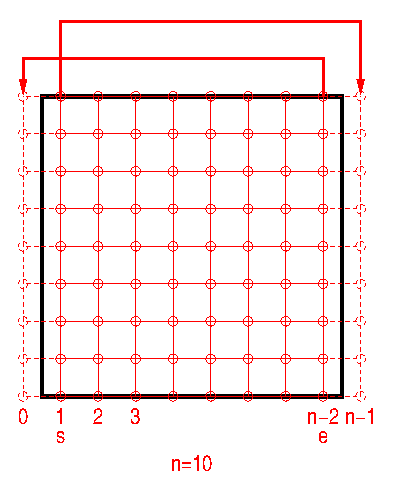
\includegraphics[scale=0.85]{Figures/Edge/1periodic_1sequential_2patterns.eps}}
  \end{picture}
  \caption{Communication patterns for sequential edge-based variable with 
           periodic boundary condition.}
  \label{edge:112}
\end{figure}

Description of Fig.~\ref{edge:112}: Same as for Fig.~\ref{cell:112}.

%%%%%%%%%%%%%%%%%%%%%%%
%                     %
%  Parallel Periodic  %
%                     %
%%%%%%%%%%%%%%%%%%%%%%%
\clearpage
\subsection{Parallel Periodic}

\subsubsection{Numeration}

%-------------%
%             %
% Edge 1.2.1. %
%             %
%-------------%
\begin{figure}[ht]
  \centering
  \setlength{\unitlength}{1mm}
  \begin{picture}(105,145)(0,0)
    \thickbox{105}{145}
    \put( 1,0){\includegraphics[scale=0.85]{Figures/Edge/1periodic_2parallel_1numeration.eps}}
  \end{picture}
  \caption{Numeration of edge-based variable with periodic boundary 
           condition for parallel computation.}
  \label{edge:121}
\end{figure}

Description of Fig.~\ref{edge:121}: Same as for Fig.~\ref{cell:121}.

\clearpage
\subsubsection{Communication}

%-------------%
%             %
% Edge 1.2.2. %
%             %
%-------------%
\begin{figure}[ht]
  \centering
  \setlength{\unitlength}{1mm}
  \begin{picture}(105,75)(0,0)
    \thickbox{105}{75}
    \put( 1,0){\includegraphics[scale=0.85]{Figures/Edge/1periodic_2parallel_2patterns.eps}}
  \end{picture}
  \caption{Communication patterns for parallel edge-based variable with 
           periodic boundary condition.}
  \label{edge:122}
\end{figure}

Description of Fig.~\ref{edge:122}: Same as for Fig.~\ref{cell:122}.

%%%%%%%%%%%%%%%%%%%%%%%%%%%%%
%                           %
%  Sequential Non-periodic  %
%                           %
%%%%%%%%%%%%%%%%%%%%%%%%%%%%%
\subsection{Sequential Non-periodic}

\subsubsection{Numeration}

%-------------%
%             %
% Edge 2.1.1. %
%             %
%-------------%
\begin{figure}[ht]
  \centering
  \setlength{\unitlength}{1mm}
  \begin{picture}(105,70)(0,0)
    \thickbox{105}{70}
    \put( 1,0){\includegraphics[scale=0.85]{Figures/Edge/2non-periodic_1sequential_1numeration.eps}}
  \end{picture}
  \caption{Numeration of sequential edge-based variable with non-periodic boundary
           condition.}
  \label{edge:211}
\end{figure}

Description of Fig.~\ref{edge:211}: Same as for Fig.~\ref{cell:211}.

%%%%%%%%%%%%%%%%%%%%%%%%%%%
%                         %
%  Parallel Non-periodic  %
%                         %
%%%%%%%%%%%%%%%%%%%%%%%%%%%
\subsection{Parallel Non-periodic}

\subsubsection{Numeration}

%-------------%
%             %
% Edge 2.2.1. %
%             %
%-------------%
\begin{figure}[ht]
  \centering
  \setlength{\unitlength}{1mm}
  \begin{picture}(105,145)(0,0)
    \thickbox{105}{145}
    \put( 1,0){\includegraphics[scale=0.85]{Figures/Edge/2non-periodic_2parallel_1numeration.eps}}
  \end{picture}
  \caption{Numeration of sequential edge-based variable with non-periodic boundary
           condition.}
  \label{edge:221}
\end{figure}

Description of Fig.~\ref{edge:221}: Same as for Fig.~\ref{cell:221}.

\clearpage
\subsubsection{Communication}

%-------------%
%             %
% Edge 2.2.2. %
%             %
%-------------%
\begin{figure}[ht]
  \centering
  \setlength{\unitlength}{1mm}
  \begin{picture}(105,65)(0,0)
    \thickbox{105}{65}
    \put( 1,0){\includegraphics[scale=0.85]{Figures/Edge/2non-periodic_2parallel_2patterns.eps}}
  \end{picture}
  \caption{Communication patterns for parallel edge-based variable with 
           periodic boundary condition.}
  \label{edge:222}
\end{figure}

Description of Fig.~\ref{edge:222}: Same as for Fig.~\ref{cell:222}.

%------------------------------------------------------------------------notes-%
\vspace*{5mm} \fbox{ \begin{minipage}[c] {0.97\textwidth} %--------------notes-%
    {\sf Note on other coordinate directions} \\ %-----------------------notes-%

Edge-based variables have the same numeration and communication patterns as
cell-based ones, but the other two directions must be treated like node-based
variables explained in Sec.~\ref{sec:node-based}.

  \end{minipage} } %-----------------------------------------------------notes-%
%------------------------------------------------------------------------notes-%

  \clearpage
\section{Summary}
\label{sec:summary}

This section summarizes all possible variable arrangements and their dimensions
in {\psiboil}. {\em Offsets} for communication buffers are also included. 

\begin{large}
\begin{center}
\begin{tabular}{ l l|l|l|l|l|l|l|}
  \cline{3-8}
                                                               % column 1
      &                                                        % column 2
          & \multicolumn{3}{c|}{\sf Resolution}                % column 3,4,5 
              & \multicolumn{3}{c|}{\sf Offset}            \\  % column 6,7,8
%------------------------------------------------------------------------------%
                                                               % column 1
      &                                                        % column 2
          &   $i$   &   $i$   &   $k$                          % column 3,4,5
              &   $i$   &   $j$   &   $k$                  \\  % column 6,7,8
%------------------------------------------------------------------------------%
  \cline{3-8} %----------------------------------------------------------------%
  \hline      %----------------------------------------------------------------%
%------------------------------------------------------------------------------%
  \multicolumn{1}{|l}{\sf User-defined}                        % column 1
      &                                                        % column 2
          &   $N_i$   &   $N_j$   &   $N_k$                    % column 3,4,5
              &   0   &   0   &   0                        \\  % column 6,7,8
%------------------------------------------------------------------------------%
  \hline      %----------------------------------------------------------------%
  \hline      %----------------------------------------------------------------%
%------------------------------------------------------------------------------%
  \multicolumn{1}{|l}{\sf Cell-based}                          % column 1
      &   $\phi$                                               % column 2
          &   $n_i=N_i+2$   &   $n_j=N_j+2$   &   $n_k=N_k+2$  % column 3,4,5
              &   0   &   0   &   0                        \\  % column 6,7,8
%------------------------------------------------------------------------------%
  \hline      %----------------------------------------------------------------%
  \hline      %----------------------------------------------------------------%
%------------------------------------------------------------------------------%
  \multicolumn{1}{|l}{\multirow{3}{*}{\sf Face-based}}         % column 1
      &   $u_i$                                                % column 2
          &   $n_i+1$ &   $n_j$   &   $n_k$                    % column 3,4,5
              &   1   &   0   &   0                        \\  % column 6,7,8
  \cline{2-8} %----------------------------------------------------------------%
  \multicolumn{1}{|c}{}                                        % column 1 
      &   $u_j$                                                % column 2
          &   $n_i$ &   $n_j+1$   &   $n_k$                    % column 3,4,5
              &   0   &   1   &   0                        \\  % column 6,7,8
  \cline{2-8} %----------------------------------------------------------------%
  \multicolumn{1}{|c}{}                                        % column 1
      &   $u_k$                                                % column 2
          &   $n_i$ &   $n_j$   &   $n_k+1$                    % column 3,4,5
              &   0   &   0   &   0                        \\  % column 6,7,8
%------------------------------------------------------------------------------%
  \hline      %----------------------------------------------------------------%
  \hline      %----------------------------------------------------------------%
%------------------------------------------------------------------------------%
  \multicolumn{1}{|l}{\sf Node-based}                          % column 1
      &   $f$                                                  % column 2
          &   $n_i+1$   &   $n_j+1$   &   $n_k+1$              % column 3,4,5
              &   1   &   1   &   1                        \\  % column 6,7,8
%------------------------------------------------------------------------------%
  \hline      %----------------------------------------------------------------%
  \hline      %----------------------------------------------------------------%
%------------------------------------------------------------------------------%
  \multicolumn{1}{|l}{\multirow{3}{*}{\sf Edge-based}}         % column 1
      &   $\sigma_i$                                           % column 2
          &   $n_i$ &   $n_j+1$   &   $n_k+1$                  % column 3,4,5
              &   0   &   1   &   1                        \\  % column 6,7,8
  \cline{2-8} %----------------------------------------------------------------%
  \multicolumn{1}{|c}{}                                        % column 1 
      &   $\sigma_j$                                           % column 2
          &   $n_i+1$ &   $n_j$   &   $n_k+1$                  % column 3,4,5
              &   1   &   0   &   1                        \\  % column 6,7,8
  \cline{2-8} %----------------------------------------------------------------%
  \multicolumn{1}{|c}{}                                        % column 1
      &   $\sigma_k$                                           % column 2
          &   $n_i+1$ &   $n_j+1$   &   $n_k$                  % column 3,4,5
              &   1   &   1   &   0                        \\  % column 6,7,8
%------------------------------------------------------------------------------%
  \hline      %----------------------------------------------------------------%
%------------------------------------------------------------------------------%
\end{tabular}
\end{center}
\end{large}


% \end{document}


  \chapter{Time-stepping}
  This section explains the implementation of time-stepping 
(time-integration) algorithms in {\psiboil}. Since {\psiboil} supports variety
of time-stepping schemes, this is far from an easy task. To make matters 
even more complex, the implementation spans over several objects and member 
functions. 

Therefore, it is strongly recommended that the reader prints the following 
functions:
%
\begin{itemize}
  \item {\tt Src/Ravioli/timescheme.h}
  \item {\tt Src/Equation/equation.h}
  \item {\tt Src/Equation/Centered/centered.h}
  \item {\tt Src/Equation/Centered/centered\_new\_time\_step.cpp}
  \item {\tt Src/Equation/Centered/centered\_update\_rhs.cpp}
  \item {\tt Src/Equation/Centered/centered\_solve.cpp}
\end{itemize}
%
and keeps the printouts at hand while reading this chapter.

This chapter begins with a recollection of the conservation equation for 
general variable. This is done in order to identify different terms in the
governing equations, their possible time time-discretization schemes and 
relation to the final form of the discretized system of equations.

The section which follows focuses on implementation of these concepts into
{\psiboil}. In order to do that, two objects had to be explained in more
details {\tt TimeScheme} which is a ravioli object holding basic information
on time-stepping schemes and {\tt Centered} which embodies the implementation
of time-stepping schemes. Everything what is explained about the {\tt Centered}
class is also valid for its children, as well as for its sister 
class~{\tt Staggered}. 

  \section{Recollection of some basic concepts}
\label{sec:recollection}

\subsection{General conservation equation}

\noindent
Integral equation for conservation of a general variable reads:
%
\be
  \frac{\p}{\p t} \int_V ( \rho B_\phi \phi ) dV  
  + 
  \oint_S ( \rho B_\phi \uvw \phi ) dS
  = 
  \oint_S  (\Gamma_\phi \nabla \phi ) dS
  +
  \int_V f_\phi dV
\ee
%
If, for the sake of shortness, we introduce the following definitions:
%
\bea
  \mathbb{Q}_\phi & = & \int_V ( \rho B_\phi \phi ) dV         \\ 
  \mathbb{H}_\phi & = & \oint_S ( \rho B_\phi \uvw \phi ) dS   \\ 
  \mathbb{D}_\phi & = & \oint_S  (\Gamma_\phi \nabla \phi ) dS \\
  \mathbb{F}_\phi & = & \int_V f_\phi dV
\eea
%
where $\mathbb{Q}_\phi$ represents the {\em innertial} term, $\mathbb{H}_\phi$ 
the {\em advection}, $\mathbb{D}_\phi$ the {\em diffusion} and 
$\mathbb{F}_\phi$ the {\em forcing} (source) term, the conservation equation 
for a general variable assumes the form:
%
\be
  \frac{\p}{\p t} \mathbb{Q}_\phi + \mathbb{H}_\phi 
  = 
  \mathbb{D}_\phi + \mathbb{F}_\phi
\ee

\subsection{Integration in time}

As the next step, this equation is discretized in time. In order to do that,
it is worthwhile introducing convention on time steps:
\begin{itemize}
  \item {\em New time step}~($N$) is the one which is currently being resolved, 
        i.e.\ the one whose value is unknown. 
  \item {\em Old time step}~($N-1$) represents the time step before new, hence
        it is the last known quantity, and
  \item {\em Very old time step}~($N-2$) is the time step before old.
\end{itemize}
%
In {\psiboil}, a linear variation between the new~($N$) and the old~($N-1$) time 
step is assumed for the innertial term, expressed as:
%
\be
  \frac{\p}{\p t} \mathbb{Q}_\phi 
  = 
  \frac{\mathbb{Q}^N_\phi - \mathbb{Q}^{N-1}_\phi}{\Delta t}
\ee

For advection, diffusion and forcing term different options exist. First order
{\em backward Euler} (fully implicit) discretization for all terms is expressed 
as:
%
\be
  \frac{\mathbb{Q}^N_\phi - \mathbb{Q}^{N-1}_\phi}{\Delta t}
  +
  \mathbb{H}^N_\phi
  =
  \mathbb{D}^N_\phi
  +
  \mathbb{F}^N_\phi.
\ee
%
This scheme is famous for its stability. 
First order {\em forward Euler} (fully explicit) scheme for all terms reads:
%
\be
  \frac{\mathbb{Q}^N_\phi - \mathbb{Q}^{N-1}_\phi}{\Delta t}
  +
  \mathbb{H}^{N-1}_\phi
  =
  \mathbb{D}^{N-1}_\phi
  +
  \mathbb{F}^{N-1}_\phi.
\ee
%
and its most advantages feature is simplicity. Second order, semi-implicit
{\em Crank-Nicolson} for all terms reads:
%
\be
  \frac{\mathbb{Q}^N_\phi - \mathbb{Q}^{N-1}_\phi}{\Delta t}
  +
  \frac{1}{2}\mathbb{H}^{N}_\phi
  +
  \frac{1}{2}\mathbb{H}^{N-1}_\phi
  =
  \frac{1}{2}\mathbb{D}^{N}_\phi
  +
  \frac{1}{2}\mathbb{D}^{N-1}_\phi
  +
  \frac{1}{2}\mathbb{F}^{N}_\phi
  +
  \frac{1}{2}\mathbb{F}^{N-1}_\phi
\ee
%
Very often, different schemes are used for different terms. If advection
terms are treated with {\em Adams-Bashforth}, diffusive with Crank-Nicolson and
forcing terms with forward Euler, the equations would read:
%
\be
  \frac{\mathbb{Q}^N_\phi - \mathbb{Q}^{N-1}_\phi}{\Delta t}
  +
  \frac{3}{2}\mathbb{H}^{N-1}_\phi
  -
  \frac{1}{2}\mathbb{H}^{N-2}_\phi
  =
  \frac{1}{2}\mathbb{D}^{N}_\phi
  +
  \frac{1}{2}\mathbb{D}^{N-1}_\phi
  +
  \mathbb{F}^{N-1}_\phi
\ee
%
This is a very often choice in {\psiboil} simulations, as Adams-Bashforth offers
simplicity for non-linear advection terms, while Crank-Nicolson gives 
stability to linear diffusive terms. 

\subsection{Discretized system of equations}

\noindent
The final result of discretization procedure is a linear system of equations:
%
\be
  [A] \cdot \{\phi^N\} = \{f\}
\ee
%
where $[A]$ represents the system matrix, $\{\phi^N\}$
is the unknown vector at new time step $N$ and $\{f\}$ the right-hand side. 
System matrix contains contribution from inertial and implicit part of the 
diffusion terms, while the right hand side contains everything else: advection 
terms, source terms and explicitly treated diffusive terms. This is illustrated 
in Table~\ref{tbl:system}.
%
\begin{table}[h!]
  \begin{center}
    \begin{tabular}{cc|c|c|}
    \cline{3-3}
    & & \multicolumn{1}{ c|}{Contains contribution from:} \\ 
    \cline{1-3}
    \multicolumn{1}{|c|}{\multirow{3}{*}{Term:}} &
    \multicolumn{1}{ c|}{$[A]$}        & $\mathbb{Q}^N/\Delta t$, 
                                         $\mathbb{D}^N$   \\ 
    \cline{2-3}
    \multicolumn{1}{|c|}{}                        &
    \multicolumn{1}{ c|}{$\{\phi^N\}$} & -         \\ 
    \cline{2-3}
    \multicolumn{1}{|c|}{}                        &
    \multicolumn{1}{ c|}{$\{f\}$}      & $\mathbb{Q}^{N-1}/\Delta t$,
                                         $\mathbb{D}^{N-1}$,    
                                         $\mathbb{H}^{N}$,    
                                         $\mathbb{H}^{N-1}$,    
                                         $\mathbb{H}^{N-2}$,    
                                         $\mathbb{F}$   \\ 
    \cline{1-3}
    \end{tabular}
    \caption{Dependence of linear system of equation on various terms
             in the governing equation.}
    \label{tbl:system}
  \end{center}
\end{table}
%

In Table~\ref{tbl:system} it is asssumed that system matrix does not change 
in time and no assumption on time discretization of the external source 
term~($\mathbb{F}$) is done.

  \section{Implementation in {\psiboil}}
\label{sec:implementation}

\subsection{Storing information on time-stepping scheme}

In a computer program one needs a way to impose and control the time stepping 
schemes. In {\psiboil}, it is achieved with the ravioli object {\tt TimeScheme} 
defined in {\tt Src/Ravioli}. From {\em user} point of view, one adjusts the 
desired time stepping scheme in the main function. 
For example, program ({\tt 07-01-main.cpp}) from Volume~1 of the tutorial, 
defines the enthalpy conservation equation and sets the time stepping scheme
for diffusion as:
%
{\small \begin{verbatim}
     29
     30   Enthalpy enth(t, q, uvw, time, solver, &solid);   /* enthalpy conservation
     31                                                        equation              */
     32   enth.diffusion_set(TimeScheme::backward_euler()); /* time stepping scheme */
     33
\end{verbatim}}
%
A {\tt TimeScheme} object has three member functions: {\tt N()}, {\tt Nm1()} 
and~{\tt Nm2()} which hold the coefficients multiplying time levels at $N$, 
$N-1$ and~$N-2$ respectively.
%
Table~\ref{tbl:schemes} illustrates this point by summarizing values member
functions return, depending on the time-stepping scheme.
%
\begin{table}[h!]
  \begin{center}
    \begin{tabular}{rr|c|c|c|c|l}
      \cline{3-5}
        &  & \multicolumn{3}{ c|}{Function:}       \\ 
      \cline{3-5}
        &  & {\tt N()} & {\tt Nm1()} & {\tt Nm2()} \\ 
      \cline{1-5}
      \multicolumn{1}{|c|}{\multirow{4}{*}{\tt TimeScheme::}} &
      \multicolumn{1}{ c|}{\tt backward\_euler()}  &  1  &  0  &  0   \\ \cline{2-5}
      \multicolumn{1}{|c|}{}                   &
      \multicolumn{1}{ c|}{\tt forward\_euler()}   &  0  &  1  &  0   \\ \cline{2-5}
      \multicolumn{1}{|c|}{}                   &
      \multicolumn{1}{ c|}{\tt crank\_nicolson()}  & 1/2 & 1/2 &  0   \\ \cline{2-5}
      \multicolumn{1}{|c|}{}                   &
      \multicolumn{1}{ c|}{\tt adams\_bashforth()} &  0  & 3/2 &-1/2   \\ \cline{1-5}
    \end{tabular}
    \caption{Values of member functions {\tt N()}, {\tt Nm1()} and~{\tt Nm2()} for 
             different time-stepping schemes.}
    \label{tbl:schemes}
  \end{center}
\end{table}

\subsection{Implementation of the time-stepping algorithms}

\noindent
From {\em development} point of view, {\tt TimeScheme}s are contained in object 
{\tt Equation}, as shown with an excerpt from the file 
{\tt equation.h}:
%
{\small \begin{verbatim}
     42
     43   protected:
     44     TimeScheme diff_ts;
     45     TimeScheme conv_ts;
\end{verbatim}}
%
So, there are two objects of type {\tt TimeScheme} defined inside {\tt Equation}
called {\tt conv\_ts} and {\tt diff\_ts} which define time-stepping schemes for
advection and diffusion terms. Their default values are set in the constructor,
as shown in lines 26--27 of the same file:
%
{\small \begin{verbatim}
     18 class Equation {
     19   public:
     20     Equation(const Domain * d,
     21              const Times  * t,
     22              Matter * f,
     23              Matter * s,
     24              Krylov * sm) :
     25       dom(d), time(t), flu(f), sol(s), solver(sm),
     26       conv_ts(TimeScheme::adams_bashforth()),
     27       diff_ts(TimeScheme::crank_nicolson()),
     28       lim(ConvScheme::superbee()) {}
\end{verbatim}}
%
As this constructor shows, the default scheme for advection is Adams-Bashforth
and for diffusion is Crank-Nicolson.  

Objects {\tt Centered} and {\tt Staggered} store parts of the linear system of
equations in: {\tt Matrix A} which holds the system matrix~$[A]$, {\tt phi} 
holding the variable~$\{\phi\}$ and {\tt Scalar fnew} holding the right hand
side~$\{f\}$. In addition, {\tt Scalars} {\tt fold}, {\tt cnew}, {\tt cold}
are used for storing intermediate parts of right-hand side.

\subsubsection{Non-iterative time-advancement}

Let's take the program {\tt 09-02-main.cpp} from the Volume~1 tutorial and
focus only on the solution of enthalpy equation. A fraction of the 
{\tt 09-02-main.cpp} is included below:
%
{\small \begin{verbatim}
     77   Enthalpy enth( t,   g,   uvw, time, solver, &fluid);
     ...
     83   for(time.start(); time.end(); time.increase()) {
     ...
     93     enth.new_time_step();
     94     enth.solve(ResRat(0.001));
     ...
\end{verbatim}}
%
Line 77 defines the equation for enthalpy, line~83 starts the time loop and
lines~93 and~94 are all that is needed to advance enthalpy in time for
non-iterative algorithms. 
Since the time-stepping schemes was not changed for {\tt Enthalpy}, it uses the 
default settings which is Adams-Bashforth for advection and Crank-Nicolson for 
diffusion.
%
When a new time step begins (after line~83), data members from {\tt Centered} 
contain the following:
%
  \begin{center}
    \begin{tabular}{cc|c|cc}
    \cline{3-3}
    & & \multicolumn{1}{ c|}{Holds:} & \\ 
    \cline{1-3}
    \multicolumn{1}{|c|}{\multirow{3}{*}{Member:}} &
    \multicolumn{1}{ l|}{\tt Matrix A}   & $[A]$ &      \\ 
    \cline{2-3}
    \multicolumn{1}{|l|}{} &
    \multicolumn{1}{ l|}{\tt Scalar phi} & $\{\phi^{N-1}\}$ & \\ 
    \cline{2-3}
    \multicolumn{1}{|l|}{} &
    \multicolumn{1}{ l|}{\tt Scalar cold} & $\mathbb{H}^{N-2} $ & \\
    \cline{1-3}
    \end{tabular}
  \end{center}
%
The reason why {\tt cold} contains $\mathbb{H}^{N-2}$ will be clear by the 
end of this section.

With these values we enter {\tt Centered::new\_time\_step()} function, defined 
in {\tt centered\_new\_time\_step.cpp}, outlined below:
%
{\small \begin{verbatim}
     ...
     13 void Centered::new_time_step() {
     ...
     23   /* no transport in solid */
     24   if( !solid() )
     25     for_ijk(i,j,k) {
     26       const real c = fluid()->cp (i,j,k);
     27       const real r = fluid()->rho(i,j,k);
     28
     29       fold[i][j][k] = r * c * dV(i,j,k) * phi[i][j][k] * time->dti()
     30                     + conv_ts.Nm2() * cold[i][j][k];  
     31     }
     ...
     53   /* a condition like: if(conv_ts != backward_euler()) would be good */
     54   convection(&cold);
     55   for_ijk(i,j,k)
     56     fold[i][j][k] += conv_ts.Nm1() * cold[i][j][k]; /* conv_ts.Nm1() = 1.5 */
     ...
     63   /* a condition like: if(diff_ts != backward_euler()) would be good */
     64   diffusion();
     ...
\end{verbatim}}
%
Lines 25--31 update the right-hand side with the part of the unsteady term from
time step~$N-1$ and advection term from time step $N-2$. After line~31, data 
members hold the following:
%
  \begin{center}
    \begin{tabular}{cc|c|cc}
    \cline{3-3}
    & & \multicolumn{1}{ c|}{Holds:} & \\ 
    \cline{1-3}
    \multicolumn{1}{|c|}{\multirow{4}{*}{Member:}} &
    \multicolumn{1}{ l|}{\tt Matrix A}   & $[A]$ &      \\ 
    \cline{2-3}
    \multicolumn{1}{|l|}{} &
    \multicolumn{1}{ l|}{\tt Scalar phi} & $\{\phi^{N-1}\}$ & \\ 
    \cline{2-3}
    \multicolumn{1}{|l|}{} &
    \multicolumn{1}{ l|}{\tt Scalar fold} & $\mathbb{Q}^{N-1}/\Delta t$,
                                            $\mathbb{H}^{N-2} $ & $\gets$ change \\
    \cline{2-3}
    \multicolumn{1}{|l|}{} &
    \multicolumn{1}{ l|}{\tt Scalar cold} & $\mathbb{H}^{N-2} $ & \\
    \cline{1-3}
    \end{tabular}
  \end{center}
%
Line~54 calls member function {\tt convection} which computes the advection
term with the last available velocity and stores it into member {\tt cnew}.
In the present case, last available velocity is the one from the previous
time step ($N-1$), so function {\tt convection} will 
compute~$\mathbb{H}^{N-1}$. Therefore, after the line~54, data members have 
contain the following:
%
  \begin{center}
    \begin{tabular}{cc|c|cc}
    \cline{3-3}
    & & \multicolumn{1}{ c|}{Holds:} & \\ 
    \cline{1-3}
    \multicolumn{1}{|c|}{\multirow{4}{*}{Member:}} &
    \multicolumn{1}{ l|}{\tt Matrix A}   & $[A]$ &      \\ 
    \cline{2-3}
    \multicolumn{1}{|l|}{} &
    \multicolumn{1}{ l|}{\tt Scalar phi} & $\{\phi^{N-1}\}$ & \\ 
    \cline{2-3}
    \multicolumn{1}{|l|}{} &
    \multicolumn{1}{ l|}{\tt Scalar fold} & $\mathbb{Q}^{N-1}/\Delta t$,
                                            $\mathbb{H}^{N-2} $ & \\
    \cline{2-3}
    \multicolumn{1}{|l|}{} &
    \multicolumn{1}{ l|}{\tt Scalar cold} & $\mathbb{H}^{N-1} $ & $\gets$ change \\
    \cline{1-3}
    \end{tabular}
  \end{center}
%
Lines~55 and~56 update the right hand side with advection from previous time
step. Thus, after line 56 data members hold the following:
%
  \begin{center}
    \begin{tabular}{cc|c|cc}
    \cline{3-3}
    & & \multicolumn{1}{ c|}{Holds:} & \\ 
    \cline{1-3}
    \multicolumn{1}{|c|}{\multirow{4}{*}{Member:}} &
    \multicolumn{1}{ l|}{\tt Matrix A}   & $[A]$ &      \\ 
    \cline{2-3}
    \multicolumn{1}{|l|}{} &
    \multicolumn{1}{ l|}{\tt Scalar phi} & $\{\phi^{N-1}\}$ & \\ 
    \cline{2-3}
    \multicolumn{1}{|l|}{} &
    \multicolumn{1}{ l|}{\tt Scalar fold} & $\mathbb{Q}^{N-1}/\Delta t$,
                                            $\mathbb{H}^{N-2}$,
                                            $\mathbb{H}^{N-1}$ & $\gets$ change \\
    \cline{2-3}
    \multicolumn{1}{|l|}{} &
    \multicolumn{1}{ l|}{\tt Scalar cold} & $\mathbb{H}^{N-1} $ & \\
    \cline{1-3}
    \end{tabular}
  \end{center}
%
Line~64 calls member function {\tt diffusion} which updates {\tt fold}
with the explicitly treated part of the diffusion term. After line~64
data members have the following meaning:
%
  \begin{center}
    \begin{tabular}{cc|c|cc}
    \cline{3-3}
    & & \multicolumn{1}{ c|}{Holds:} & \\ 
    \cline{1-3}
    \multicolumn{1}{|c|}{\multirow{4}{*}{Member:}} &
    \multicolumn{1}{ l|}{\tt Matrix A}   & $[A]$ &      \\ 
    \cline{2-3}
    \multicolumn{1}{|l|}{} &
    \multicolumn{1}{ l|}{\tt Scalar phi} & $\{\phi^{N-1}\}$ & \\ 
    \cline{2-3}
    \multicolumn{1}{|l|}{} &
    \multicolumn{1}{ l|}{\tt Scalar fold} & $\mathbb{Q}^{N-1}/\Delta t$,
                                            $\mathbb{H}^{N-2}$,
                                            $\mathbb{H}^{N-1}$,
                                            $\mathbb{D}^{N-1}$ & $\gets$ change \\
    \cline{2-3}
    \multicolumn{1}{|l|}{} &
    \multicolumn{1}{ l|}{\tt Scalar cold} & $\mathbb{H}^{N-1} $ & \\
    \cline{1-3}
    \end{tabular}
  \end{center}
%
Data members hold the same meaning when exiting from the {\tt new\_time\_step}
function. After the call to {\tt new\_time\_step} in the main function, a call
to {\tt solve} is issued. Part of the {\tt Centered::solve()}, defined in
{\tt centered\_solve.cpp}, is given below:
%
{\small \begin{verbatim}
     ...
      9 void Centered::solve(const real & fact, const char * name) {
     ...
     23   /* solve */
     24   update_rhs();
     25   solver->solve(A, phi, fnew, 20, name);
     ...
\end{verbatim}}
%
and shows that a call to {\tt Centered::update\_rhs()} is performed in line~24,
just before staring the linear solver in line~25. As its name implies, this 
function updates the right-hand side, as the portion of the code, located in
{\tt centered\_update\_rhc.cpp} shows:
%
{\small \begin{verbatim}
     12 real Centered::update_rhs() {
     ...
     19   for_ijk(i,j,k) {
     20     fnew[i][j][k] = fold[i][j][k]
     21                   + cnew[i][j][k] * conv_ts.N()
     22                   + fbnd[i][j][k]
     23                   + fext[i][j][k];
     24   }
     ...
\end{verbatim}}
%
As lines~19--24 show, this function fills the right hand side with all the 
terms needed. After the {\tt Centered::update\_rhs()}, which is also just
before calling the liner solver at line~25 in {\tt Centered::solve()}, 
data members hold the following:
%
  \begin{center}
    \begin{tabular}{cc|c|cc}
    \cline{3-3}
    & & \multicolumn{1}{ c|}{Holds:} & \\ 
    \cline{1-3}
    \multicolumn{1}{|c|}{\multirow{4}{*}{Member:}} &
    \multicolumn{1}{ l|}{\tt Matrix A}   & $[A]$ &      \\ 
    \cline{2-3}
    \multicolumn{1}{|l|}{} &
    \multicolumn{1}{ l|}{\tt Scalar phi} & $\{\phi^{N-1}\}$ & \\ 
    \cline{2-3}
    \multicolumn{1}{|l|}{} &
    \multicolumn{1}{ l|}{\tt Scalar fnew} & $\mathbb{Q}^{N-1}/\Delta t$,
                                            $\mathbb{H}^{N-2}$,
                                            $\mathbb{H}^{N-1}$,
                                            $\mathbb{D}^{N-1}$,  
                                            $\mathbb{F}$ & $\gets$ change \\
    \cline{2-3}
    \multicolumn{1}{|l|}{} &
    \multicolumn{1}{ l|}{\tt Scalar fold} & $\mathbb{Q}^{N-1}/\Delta t$,
                                            $\mathbb{H}^{N-2}$,
                                            $\mathbb{H}^{N-1}$,
                                            $\mathbb{D}^{N-1}$ & \\
    \cline{2-3}
    \multicolumn{1}{|l|}{} &
    \multicolumn{1}{ l|}{\tt Scalar cold} & $\mathbb{H}^{N-1} $ & \\
    \cline{1-3}
    \end{tabular}
  \end{center}
%
Note that, although line~21 in {\tt centered\_update\_rhc.cpp}
adds contribution from {\tt cnew}, it is also multiplied by {\tt conv\_ts.N()},
which is equal to zero for non-iterative time-stepping schemes. 

At this stage, {\tt fnew} holds all the contributions it needs and a call to 
linear solver can be performed, which yields new value of dependent variable.
Hence, after the call to solver, data members contain the following:
%
  \begin{center}
    \begin{tabular}{cc|c|cc}
    \cline{3-3}
    & & \multicolumn{1}{ c|}{Holds:} & \\ 
    \cline{1-3}
    \multicolumn{1}{|c|}{\multirow{5}{*}{Member:}} &
    \multicolumn{1}{ l|}{\tt Matrix A}   & $[A]$ &      \\ 
    \cline{2-3}
    \multicolumn{1}{|l|}{} &
    \multicolumn{1}{ l|}{\tt Scalar phi} & $\{\phi^N\}$ & $\gets$ change \\ 
    \cline{2-3}
    \multicolumn{1}{|l|}{} &
    \multicolumn{1}{ l|}{\tt Scalar fnew} & $\mathbb{Q}^{N-1}/\Delta t$,
                                            $\mathbb{H}^{N-2}$,
                                            $\mathbb{H}^{N-1}$,
                                            $\mathbb{D}^{N-1}$,  
                                            $\mathbb{F}$ &  \\
    \cline{2-3}
    \multicolumn{1}{|l|}{} &
    \multicolumn{1}{ l|}{\tt Scalar fold} & $\mathbb{Q}^{N-1}/\Delta t$,
                                            $\mathbb{H}^{N-2}$,
                                            $\mathbb{H}^{N-1}$,
                                            $\mathbb{D}^{N-1}$ & \\
    \cline{2-3}
    \multicolumn{1}{|l|}{} &
    \multicolumn{1}{ l|}{\tt Scalar cold} & $\mathbb{H}^{N-1} $ & \\
    \cline{1-3}
    \end{tabular}
  \end{center}
%
The first three members outlined above ({\tt Matrix A}, {\tt Scalar phi} and
{\tt Scalar fnew}) contain the same entries outlined in Table~\ref{tbl:system},
meaning the linear system for the governing equation is discretized properly. 

As soon as the computation of new time step starts, values in~{\tt phi} and 
{\tt cold} get older by one time level and become~$\{\phi^{N-1}\}$ 
and~$\mathbb{H}^{N-2}$ respectively. That explains the contents of the first
table in this section. 

\subsubsection{Iterative time-advancement}

The algorithm outlined above works for non-iterative time-integration algorithms
such as the projection method. For some simulations an iterative algorithm is 
required for stronger coupling of momentum and pressure, of for implicit 
treatment of non-linear or source terms. The most wide-spread iterative 
time-stepping scheme is the SIMPLE algorithm. An example of a SIMPLE-like
iterative scheme is given in the file {\tt Tests/simple/main-simple.cpp}.
A portion of the file pertinent to time-integration is given below:
%
{\small \begin{verbatim}
     ...
     96   for(time.start(); time.end(); time.increase()) {
     ...
    106     /* momentum */
    107     ns.cfl_max();
    108     ns.new_time_step();
    109
    110     // NEW: SIMPLE ITERATIONS
    111     for(int in=0; in<6; in++) {
     ...                         
    113       ns.convection();
    114       ns.solve(ResRat(0.0001));
    ...
\end{verbatim}}
%
In this case, we are solving momentum equations, rather than enthalpy. But that
doesn't matter, because objects {\tt Enthalpy} and {\tt Momentum} both descend
from {\tt Equation} and concepts for time integration are the same.

Iterative algorithms feature the so-called {\em outer} and {\em inner} loop. For
the present example, outer loop begins at line~96, whereas the inner begins at
line~111. Function {\tt Staggered::new\_time\_step()} is the analog of its 
sister variant {\tt Centered::new\_time\_step()}, and the local data member have 
the following meaning at the end of line~108:
%
  \begin{center}
    \begin{tabular}{cc|c|c|}
    \cline{3-3}
    & & \multicolumn{1}{ c|}{Holds:} \\ 
    \cline{1-3}
    \multicolumn{1}{|c|}{\multirow{5}{*}{Member:}} &
    \multicolumn{1}{ l|}{\tt Matrix A}   & $[A]$       \\ 
    \cline{2-3}
    \multicolumn{1}{|l|}{} &
    \multicolumn{1}{ l|}{\tt Scalar phi} & $\{\phi^{N-1}\}$  \\ 
    \cline{2-3}
    \multicolumn{1}{|l|}{} &
    \multicolumn{1}{ l|}{\tt Scalar fnew} & $\mathbb{Q}^{N-1}/\Delta t$,
                                            $\mathbb{H}^{N-2}$,
                                            $\mathbb{H}^{N-1}$,
                                            $\mathbb{D}^{N-1}$,  
                                            $\mathbb{F}$ \\
    \cline{2-3}
    \multicolumn{1}{|l|}{} &
    \multicolumn{1}{ l|}{\tt Scalar fold} & $\mathbb{Q}^{N-1}/\Delta t$,
                                            $\mathbb{H}^{N-2}$,
                                            $\mathbb{H}^{N-1}$,
                                            $\mathbb{D}^{N-1}$ \\
    \cline{2-3}
    \multicolumn{1}{|l|}{} &
    \multicolumn{1}{ l|}{\tt Scalar cold} & $\mathbb{H}^{N-1} $ \\
    \cline{1-3}
    \end{tabular}
  \end{center}
%
At this point, we enter the {\em inner} loop which contains a call to 
{\tt Momentum::convection()} at line~113. This subroutine updates {\tt cnew} 
with the advection term obtained from new velocities, i.e. velocities currently 
being iterated at time step~$N$. Data members in {\tt Momentum} now contain 
the following:
%
  \begin{center}
    \begin{tabular}{cc|c|cc}
    \cline{3-3}
    & & \multicolumn{1}{ c|}{Holds:} & \\ 
    \cline{1-3}
    \multicolumn{1}{|c|}{\multirow{6}{*}{Member:}} &
    \multicolumn{1}{ l|}{\tt Matrix A}   & $[A]$ &      \\ 
    \cline{2-3}
    \multicolumn{1}{|l|}{} &
    \multicolumn{1}{ l|}{\tt Scalar phi} & $\{\phi\}^{N-1}$  & \\ 
    \cline{2-3}
    \multicolumn{1}{|l|}{} &
    \multicolumn{1}{ l|}{\tt Scalar fnew} & $\mathbb{Q}^{N-1}/\Delta t$,
                                            $\mathbb{H}^{N-2}$,
                                            $\mathbb{H}^{N-1}$,
                                            $\mathbb{D}^{N-1}$,  
                                            $\mathbb{F}$ & \\
    \cline{2-3}
    \multicolumn{1}{|l|}{} &
    \multicolumn{1}{ l|}{\tt Scalar fold} & $\mathbb{Q}^{N-1}/\Delta t$,
                                            $\mathbb{H}^{N-2}$,
                                            $\mathbb{H}^{N-1}$,
                                            $\mathbb{D}^{N-1}$ & \\
    \cline{2-3}
    \multicolumn{1}{|l|}{} &
    \multicolumn{1}{ l|}{\tt Scalar cnew} & $\mathbb{H}^{N}   $ & $\gets$ change \\
    \cline{2-3}
    \multicolumn{1}{|l|}{} &
    \multicolumn{1}{ l|}{\tt Scalar cold} & $\mathbb{H}^{N-1} $ & \\
    \cline{1-3}
    \end{tabular}
  \end{center}
%
In the call to solver at line~114, right hand side {\tt fnew} is updated with
{\tt cnew}, so that the contents of inner variables before the call to linear
solver is:
%
  \begin{center}
    \begin{tabular}{cc|c|cc}
    \cline{3-3}
    & & \multicolumn{1}{ c|}{Stores:} & \\ 
    \cline{1-3}
    \multicolumn{1}{|c|}{\multirow{6}{*}{Member:}} &
    \multicolumn{1}{ l|}{\tt Matrix A}   & $[A]$ &      \\ 
    \cline{2-3}
    \multicolumn{1}{|l|}{} &
    \multicolumn{1}{ l|}{\tt Scalar phi} & $\{\phi^{N-1}\}$ & \\ 
    \cline{2-3}
    \multicolumn{1}{|l|}{} &
    \multicolumn{1}{ l|}{\tt Scalar fnew} & $\mathbb{Q}^{N-1}/\Delta t$,
                                            $\mathbb{H}^{N-2}$,
                                            $\mathbb{H}^{N-1}$,
                                            $\mathbb{H}^{N}$,
                                            $\mathbb{D}^{N-1}$,  
                                            $\mathbb{F}$ & $\gets$ changed \\
    \cline{2-3}
    \multicolumn{1}{|l|}{} &
    \multicolumn{1}{ l|}{\tt Scalar fold} & $\mathbb{Q}^{N-1}/\Delta t$,
                                            $\mathbb{H}^{N-2}$,
                                            $\mathbb{H}^{N-1}$,
                                            $\mathbb{D}^{N-1}$ & \\
    \cline{2-3}
    \multicolumn{1}{|l|}{} &
    \multicolumn{1}{ l|}{\tt Scalar cnew} & $\mathbb{H}^{N}   $ & \\
    \cline{2-3}
    \multicolumn{1}{|l|}{} &
    \multicolumn{1}{ l|}{\tt Scalar cold} & $\mathbb{H}^{N-1} $ & \\
    \cline{1-3}
    \end{tabular}
  \end{center}
%
which is exactly what is needed. After the call to linear solver, {\tt phi}
will hold the new value for velocities $\{\phi^N\}$, i.e.:
%
  \begin{center}
    \begin{tabular}{cc|c|cc}
    \cline{3-3}
    & & \multicolumn{1}{ c|}{Stores:} & \\ 
    \cline{1-3}
    \multicolumn{1}{|c|}{\multirow{6}{*}{Member:}} &
    \multicolumn{1}{ l|}{\tt Matrix A}   & $[A]$ &      \\ 
    \cline{2-3}
    \multicolumn{1}{|l|}{} &
    \multicolumn{1}{ l|}{\tt Scalar phi} & $\{\phi^N\}$ & $\gets$ changed \\ 
    \cline{2-3}
    \multicolumn{1}{|l|}{} &
    \multicolumn{1}{ l|}{\tt Scalar fnew} & $\mathbb{Q}^{N-1}/\Delta t$,
                                            $\mathbb{H}^{N-2}$,
                                            $\mathbb{H}^{N-1}$,
                                            $\mathbb{H}^{N}$,
                                            $\mathbb{D}^{N-1}$,  
                                            $\mathbb{F}$ & \\
    \cline{2-3}
    \multicolumn{1}{|l|}{} &
    \multicolumn{1}{ l|}{\tt Scalar fold} & $\mathbb{Q}^{N-1}/\Delta t$,
                                            $\mathbb{H}^{N-2}$,
                                            $\mathbb{H}^{N-1}$,
                                            $\mathbb{D}^{N-1}$ & \\
    \cline{2-3}
    \multicolumn{1}{|l|}{} &
    \multicolumn{1}{ l|}{\tt Scalar cnew} & $\mathbb{H}^{N}   $ & \\
    \cline{2-3}
    \multicolumn{1}{|l|}{} &
    \multicolumn{1}{ l|}{\tt Scalar cold} & $\mathbb{H}^{N-1} $ & \\
    \cline{1-3}
    \end{tabular}
  \end{center}
%

When the computation of new time step starts, values in~{\tt phi} and 
{\tt cold} get older by one time level and become~$\{\phi^{N-1}\}$ 
and~$\mathbb{H}^{N-2}$ respectively. 

\subsubsection{A note on external source terms}

The way external sources (or forces in case of momentum equation) are 
discretized in time is defined implicitly in the main function. 
If sources are estimated
at the beginning of time step using the know values from old~($N-1$) time
step, their discretization is based on forward Euler scheme. That is the 
most straight-forward approach for non-iterative schemes. 

In case iterative schemes are used, we can compute the value of the source
term inside the inner loop and thus have it based on the new~($N$) value of 
dependent variable making it a backward Euler scheme.

For multi-level schemes (Adams-Bashforth or Crank-Nicolson) one would have to
define two time level for sources in the main function and take care of their
proper computation. At the time of writing this tutorial, there are no examples
to demonstrate such an approach.

%---------------------------------------------------------------------nutshell-%
\vspace*{5mm} \fbox{ \begin{minipage}[c] {0.97\textwidth} %-----------nutshell-%
    {\sf Section \ref{sec:implementation} in a nutshell} \\ %-----nutshell-%

      - Implementation of time-stepping schemes in {\psiboil} is based on the
      following concepts:
      \begin{itemize}
        \item available time-discretization schemes are stored in objects of 
              type {\tt TimeScheme},
        \item {\em inertial} term of the governing equations is assumed to 
              vary linearly between the old ($N-1$) and the new ($N$) time step,
        \item {\em diffusion} term can be discretized in time with the 
              Crank-Nicolson, backward Euler and forward Euler schemes,
        \item {\em advection} term can be discretized in time with the 
              Adams-Bashforth, Crank-Nicolson, backward Euler and forward Euler 
              schemes,
        \item time-stepping scheme for {\em source} (or {\em force} term for 
              momentum) is done in the {\psiboil}'s main function, 
        \item objects of type {\tt Equation} and its descendants, keep various
              parts of discretized governing equations in {\tt Scalar} fields:
              {\tt fold}, {\tt fnew}, {\tt cold}, {\tt cnew},
        \item these {\tt Scalar} fields are updated across several {\tt Equation}
              descendant member functions, most notably {\tt new\_time\_step()},
              {\tt convection}, {\tt diffusion}, {\tt update\_rhs()} and {\tt solve}.
      \end{itemize}
      
  \end{minipage} } %--------------------------------------------------nutshell-%
%---------------------------------------------------------------------nutshell-%


  \printindex

\end{document}
